\documentclass[a4paper,12pt,twoside]{book}
\usepackage[english]{babel}
%\usepackage{fontspec}
%\setmainfont[
%  Ligatures=TeX,
%  Extension=.otf,
%  BoldFont=cmunbx,
%  ItalicFont=cmunti,
%  BoldItalicFont=cmunbi,
%  SlantedFont=cmunsl
%]{cmunrm}

%\usepackage{polyglossia}
%\setmainlanguage{spanish}

\usepackage[c5paper]{geometry}
%\geometry{inner=2.5cm,outer=2.5cm,bmargin=3.2cm}
%\usepackage[DIV=14,BCOR=2mm,headinclude=true,footinclude=false]{typearea}

%\usepackage{ulem} %Hace que \emph sea subrayar

%\usepackage[p,osf]{scholax}
%% T1 and textcomp are loaded by package. Change that here, if you want
%% load sans and typewriter packages here, if needed

\usepackage{ebgaramond}
%\usepackage[type1]{libertine} % Linux Libertine for zweispaltige Texte
%\usepackage{textcomp}% Required to get special symbols
\usepackage[scaled=.8]{DejaVuSansMono}% FiraMono Typewriter font
\usepackage{PTSansNarrow} 
%\gilliuscondensed
%\usepackage[sfdefault]{FiraSans}
%\usepackage{bm}% Extra bold faces
%\usepackage[lf]{carlito}

\usepackage{lettrine} %Capital letters at the beginning of a chapter
\usepackage[activate={true,nocompatibility},final,tracking=true,kerning=true,spacing=true,factor=1100,stretch=10,shrink=10]{microtype}
\SetTracking{encoding={*}, shape=sc}{-20} % versalitas menos separadas
% activate={true,nocompatibility} - activate protrusion and expansion
% final - enable microtype; use "draft" to disable
% tracking=true, kerning=true, spacing=true - activate these techniques
% factor=1100 - add 10% to the protrusion amount (default is 1000)
% stretch=10, shrink=10 - reduce stretchability/shrinkability (default is 20/20)

%\usepackage{array,multirow,booktabs,colortbl,chngcntr} % El último es para counterwithout;
\usepackage[strict]{changepage}
%\usepackage{caption}
%\captionsetup{format=plain,labelsep=newline,labelfont={small,sc},
%textfont={small,it},singlelinecheck=false}
\usepackage[Bjornstrup]{fncychap} % Para cabeceras de capítulos sofisticados:     Sonny,    Lenny,    Glenn,    Conny,    Rejne,    and Bjarne.

\usepackage{graphicx,wrapfig,booktabs,multicol} % wallpaper: poner imágenes de fondo; wrapfigure: figuras a un lado del texto
%\graphicspath{{figures/}}
\usepackage{fancyhdr}
\usepackage{emptypage,pdfpages,fancybox} % Para que las páginas en blanco no tengan encabezado;
\usepackage{enumitem} %paralist: para compactenum, enumerate sin espacios
%\setlist[itemize]{nosep} %Espacio entre items en itemize
\usepackage[hyperref]{xcolor}
\usepackage[hidelinks]{hyperref}
\usepackage{xurl,breakurl}

%\usepackage{minipage}

%\usepackage{quotchap} %Encabezados de capítulos
\usepackage{syntonly,verbatim}
%\syntaxonly

\usepackage{setspace,xspace} % xspace: Da \xspace para no tener que poner {} después de los comandos; pdflscape: páginas en horizontal;

\newenvironment{quotex}{\begin{quote}\small}{\end{quote}}
\newenvironment{quotationx}{\begin{quotation}\small}{\end{quotation}}


\begin{document}

% Por alguna razón, los marginados se creaban al revés. Así los corrijo. Feo, pero eficaz:
\let\tmp\oddsidemargin
\let\oddsidemargin\evensidemargin
\let\evensidemargin\tmp
\reversemarginpar

%\setcounter{secnumdepth}{4} % Para que llegue a numerar hasta las subsubsecciones;
%\renewcommand{\heavyrulewidth}{0.14em} % Grosor de las líneas extremas de las tablas;
%\renewcommand\thempfootnote{\alpha{mpfootnote}} % Símbolo de notas dentro de minipage
%\let\oldcaptionof\captionof
%\renewcommand{\captionof}[2]{\oldcaptionof{#1}{\newline \textit{#2} }}
%\renewcommand{\tablename}{Tabla}
%\counterwithout{figure}{chapter}
%\counterwithout{table}{chapter} % Así la numeración es 1, 2, 3... y no 1.1, 1.2... y no reinicia la num. en cada capítulo;

%\providecommand{\ggl}{\guillemotleft}
%\providecommand{\ggr}{\guillemotright\xspace}
\providecommand{\flright}[1]{\begin{flushright}#1\end{flushright}}
\providecommand{\flrightit}[1]{\begin{flushright}\itshape #1\end{flushright}}
%\renewcommand\UrlFont\sffamily
\urlstyle{tt}

\pagestyle{fancy}
\renewcommand{\sectionmark}[1]{\markright{#1}}
\renewcommand{\chaptermark}[1]{\markboth{#1}{}}

%Portada:
%\includepdf{00Portada}

\frontmatter
%
%\onehalfspacing
%\pagenumbering{Roman} %gobble es como empty

%\include{preindice}

%\fancyhf{}
%\fancyhead[LE]{\small \textbf{\thepage}$\quad$ Índice general}
%\fancyhead[RO]{\small Índice general $\quad$\textbf{\thepage}}
%\clearpage
\tableofcontents

%\doublespacing
\mainmatter

\fancyhf{}
\fancyhead[LE]{\small \thepage$\quad${\scshape\chaptername{} \thechapter}: \nouppercase{\itshape\leftmark}}
\fancyhead[RO]{\small \textsc{Section }\thesection{}: \nouppercase{\itshape\rightmark} $\quad$\upshape\thepage}
%\cfoot{\bfseries\thepage}

\pagenumbering{arabic}

%\onehalfspacing

% introductorios

\chapter{Introduction. The Path of Court Love}
\section{Lucinde}%
\label{sec:Lucinde}
\begin{quotex}
Update 12 October 2021. Thus began the path of the Knight 15 years ago, today.

\end{quotex}
From Lucinde by \textbf{Friedrich Schlegel}.

\textbf{Julius writes to Lucinde:}

\begin{quotex}
In the holy solitude around me everything was light and color, and a fresh warm breath of life and love touched me, and stirred and murmured in all the branches of the luxuriant grove. I looked, and I delighted in everything at the same time: the vigorous green, the white blossom, and the golden fruit. And so too with the eye of my spirit I saw the one and only and forever beloved in many forms: sometimes as a childlike girl, sometimes as a woman in the full bloom and strength of love and femininity, and sometimes as a worthy mother with her earnest little boy in her arms. I breathed the spring, saw clearly the eternal youthfulness around me, and I said with a smile: “Even if this world is not the best or the most useful, still I know that it is the most beautiful.”

Nothing could have shaken me in this feeling or conviction, neither general doubt nor my own fear. For I believed I was looking deeply into the secrets of nature; I felt that everything lived eternally and that even death was only an amiable deception. But, actually, I didn't think about it very much — at least I wasn't particularly disposed to classify and analyze abstract concepts.

Instead I lost myself gladly and deeply in all the comminglings and intertwinings of joy and pain from which come the savor of life and the bloom of feeling, spiritual voluptuousness as well as sensual beatitude. A subtle fire flowed in my veins; what I dreamed of wasn't just a kiss or the embrace of your arms; it wasn't just a wish to break the tormenting thorn of yearning and cool the sweet flames in surrender; I didn't yearn only for your lips or your eyes or your body.

It was, rather, a romantic confusion of all these things, a wonderful mixture of the most various memories and yearnings. All the mysteries of male and female frivolity seemed to hover about me as suddenly your real presence and the gleam of blooming happiness on your face inflamed my lonely self. Wit and rapture alternated between us and became the common pulse of our united life and we embraced each other with as much wantonness as religion.

I begged you that for once you might give yourself completely over to frenzy, and I implored you to be insatiable. Still, I listened with cool composure for every faint sign of bliss, so that not a single trace might escape me and leave a gap in our harmony. I didn't simply enjoy, but felt and enjoyed the enjoyment itself.

\end{quotex}
It may seem presumptuous to include love advice in a discussion on \emph{jnanis}, since we associate them with asceticism and celibacy. However, while it started somewhat “tongue-in-cheek”, there is a valid purpose. If non-duality is true, then every area and aspect of life is non-dual. We cannot see the ascetic as the norm — it's odd that only now are we concerned about the termination of human life on earth, whether through war or environmental destruction, when in actuality, it has always been the human prerogative to end the world simply by refusing to reproduce!

It is a sign of the times to believe we have evolved to the point of accepting practices which have traditionally been considered deviant, on the grounds that they are “natural”. However, this assumes a profound misunderstanding of man, who is anything but natural, both in a positive and a negative sense. Positively, man is more than his nature; with his source in Atman, he creates himself and cannot be reduced to biology, instinct, and impulse. To the modern mind, freedom means release from every constraint to say “yes” to every whim. However, the task of self-creation will often require a “no” instead. It will serve no point to be more specific; as in everything, prudence and wisdom will be suitable guides. Keep in mind, though, the Hermetic principle: “As above, so below”. The manifest world arises from the polarity of the male and female principles (\emph{Purusha} and \emph{Prakriti}). The most creative relationships will exhibit that polarity in the phenomenal realm.

Negatively, man does not understand his true nature. As we pointed out, his perceptions, actions, and thoughts are delusory, so man, in this unregenerate state, cannot even know his true nature, so what he considers “natural” is, from a metaphysical perspective, more likely to be the manifestation of unnatural \emph{tamasic} forces. Keep in mind that the studied “naturalness” of a Zen practitioner, or the “naturalness” of a dancer or artist, are actually the result of deep and dedicated practice.

In the past, we have quoted from \textbf{Friedrich Schlegel}`s novel \emph{Lucinde} without giving the background. Schlegel was a founder of the Romantic movement in XIXth century German art and was an innovator in bringing the Vedic teachings to Europe. The common “wisdom” among the intelligentsia at that time, was that a man needed three types of women to be fulfilled: a wife, a mistress, and an âme-soeur (soul sister). The first two are self-explanatory. But the âme-soeur is a Platonic relationship; she is able to discuss the deep things of life (e.g., art, philosophy, spirituality, etc.).

\begin{wrapfigure}{rt}{.4\textwidth}
\centering
 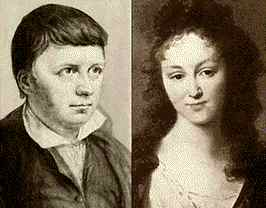
\includegraphics[scale=.5]{a20061012Lucinde-img001.jpg} 
 \caption{Friedrich and Dorothy Schlegel}
\end{wrapfigure}

Schlegel and his wife, Dorothy, turned that common wisdom on its head by incorporating all three aspects into a single relationship. The progress and results of that experiment were documented in his novel.

While the “mate” (or wife) can be seen as the public face of the relationship, the Mistress is the private face. (This is why any hint of promiscuity, adultery, exhibitionism betrays the relationship.) The public/private distinction corresponds to the exoteric/esoteric distinction in religions. So, exoterically, since sexual relations between mates is open to biological life, by correspondence, esoterically, the Mistress relationship is also open to the creation of a new life, though, in this case, it is the spiritual birth of a new being, wherein they each find their own wholeness in the other. So for Schlegel, the âme-soeur relation is not opposed to a “conventional” relationship, but is instead its fulfillment.

This extended passage from Lucinde is illustrative:

\begin{quotex}
Yes: I would have thought it a fairy tale that there could be such happiness and such love as I feel now — and such a woman, at once the most delicate lover, the most wonderful companion, and the most perfect friend. For in friendship particularly I sought for all that I lacked and didn't expect to find in any woman. In you I've found everything and even more than I could have hoped for; but, then, you're not like the others. You're untouched by the faults that custom and caprice call female. Aside from your little idiosyncrasies, the femininity of your soul consists simply in your making life and love synonymous. You feel completely and infinitely; you know of no separations; your being is one and indivisible. That is why you are so serious and so joyful. That is why you take everything so solemnly and so negligently, and also why you love me completely and don't relinquish any part of me to the state, to posterity, or to my friends.

Everything belongs to you, and we are in every respect closest to each other and understand each other best. You're at my side at every stage of human experience, from the most passionate sensuality to the most spiritual spirituality; and only in you have I seen true pride and true womanly modesty.The most extreme sorrows, if they merely enveloped us and didn't separate us, would seem to me nothing more than a refreshing contrast to the sublime frivolity of our marriage. Why shouldn't we interpret the bitterest whim of chance as a lovely witticism and an exuberant caprice, since we, like love, are immortal? I can no longer say my love or your love: both are identical and perfectly united, as much love on one side as on the other, This is marriage, the timeless union and conjunction of our spirits, not simply for what we call this world or the world beyond death, but for the one, true, indivisible, nameless, unending world, for our whole eternal life and being.
\end{quotex}
\flrightit{Posted on 2006-10-12 by Cologero }

\begin{center}* * *\end{center}

\begin{footnotesize}\begin{sffamily}



\texttt{Tannheuser on 2021-02-15 at 13:50 said: }

It may be worth meditating on whether there is a parallel between the Mother/Mistress/Ame-soeur triad and the Three Marys (John 19:25) from the New Testament. The fact that all of these important women in the New Testament are named “Mary” would seem to indicate that they are in a some sense different aspects of the same personage.

Magdalene is described as being cleansed of seven devils (Luke 8:2), and the first to behold the resurrected Christ (John 20:11-18). She is also prominent in the apocryphal and “gnostic” gospels — in the Gospel of Mary she describes exclusive and private revelations given to her by Christ, regarding the nature of the soul and spirit, and the trials the soul undergoes after death.

In all of this it's hard not think of Arcanum II of the Tarot, the High Priestess. Tomberg says that she embodies Gnosis, and if we think of Magdalene this way it makes sense that Aquinas calls her “Apostle to the Apostles”:

“Note the three privileges given to Mary Magdalene. First, she had the privilege of being a prophet because she was worthy enough to see the angels, for a prophet is an intermediary between angels and the people. Second, she had the dignity or rank of an angel insofar as she looked upon Christ, on whom the angels desire to look. Third, she had the office of an apostle; indeed, she was an apostle to the apostles insofar as it was her task to announce our Lord's resurrection to the disciples. Thus, just as it was a woman who was the first to announce the words of death, so it was a woman who would be the first to announce the words of life.” (2519)


\hfill

\texttt{Sibylle on 2023-06-05 at 03:16 said: }

Lucinde writes to Julius:

“…childlike cheerfulness and bitter pain, untamed rage and pouring dreams, death and love, desire and contemplation, sweeping exuberance and melancholy, (sweet little sighs of which none escaped my ears), dark sorrow and bright willfulness; this is what I see before me in such clear and powerful manner, gazing at me, living and striving in … letters and dreams, conversations and speeches; this is the spirit and intent of your opus, and that is why it is so dear to me, why I have taken it into my heart, out of intimate love and deep awe; it is here where I have found the clearest image of my own highest longing.”

— Fragment from the appendix of “Lucinde, Studienausgabe”, Reclam Verlag


\end{sffamily}\end{footnotesize}

\section{The Path of Courtly Love}

\begin{quotex}
neither is the man without the woman, nor the woman without the man, in the Lord. \flright{\textsc{1 Corinthians 11:11}}

\end{quotex}

\begin{quotex}
There are few people who know the full strength of the different movements of the heart. The vast majority of men are sensitive to only five or six passions in the circle in which their lives are spent and which define the boundaries of their imaginations. Take away love and hate, pleasure and pain, hope and fear, and they will feel nothing. But persons of a nobler character can be moved in thousands of different ways. It seems that they can receive ideas and sensations which surpass the ordinary norms of the common people. \flright{\textsc{Abbe Prevost}, \emph{Manon Lescaut}}

\end{quotex}
There are many paths to God — the ways of the Monk, Ascetic, Mystic, Devotee, Sage. But the most effective, and little known, may be the Way of Courtly Love. This is the path of the Fedeli d'Amore, the Troubadour, the Alchemist, and the Knight Errant. The Muslim mystic, \textbf{Ibn Arabi}, was aware of this path:

\begin{quotex}
Contemplation of God without formal support is not possible… Since therefore some form of support is necessary, the best and most perfect kind is the contemplation of God in women. 

\end{quotex}

\begin{wrapfigure}{rt}{.3\textwidth}\centering
 
\includegraphics[scale=.6]{a20210207ThePathofCourtlyLove-img001.jpg} 
\caption{Androgyne}
\end{wrapfigure}

Formal manifestation, then, is the stepping stone to formless manifestation, and ultimately to the Supreme Identity. Hence, Dante had Beatrice and Ibn Arabi had Nizam to lead them upward. I have been aware of this path since I was a young man. Although following it often brings heartache, unfortunately even to the innocent, it is nonetheless effective. Herewith, we describe some preconditions and indicate some signposts to follow along the way.

\paragraph{Emotional Education}
In the decadent parts of the modern world, great attention is paid to physical and intellectual training, while emotional development is left entirely to chance. Sure, there is talk about “emotional intelligence”, which in practice achieves nothing. There are about a half dozen primary emotions, that can even be observed in babies: delight, fear, anger, surprise, discomfort, sadness. Over time, any developments in emotional responses are usually negative: anxiety, depression, worry, despair, self-doubt, inflation. That is why esoteric training begins with some preliminary objectives:

\begin{quotex}
The chief practical objectives are mastery of the sexual center, and the training of the emotional center. \flright{\textsc{Boris Mouravieff}, \emph{Gnosis}}

\end{quotex}
Emotional problems are obstacles to the Supreme Identity as they will disappear:

\begin{quotex}
The only things which have disappeared [in the unconditioned state] are the limiting conditions, which are negative, since they represent no more than a “privation”. \flright{\textsc{Rene Guenon}, \emph{Oriental Metaphysics [OM]}} 

\end{quotex}
Otherwise, the Supreme Identity is the fulfillment all of one's potentials in his other states:

\begin{quotex}
In this unconditioned state all other states of being find their place, but they are transformed and released from the special conditions which determined them as particular states. What remains is that which has a positive reality, since herein it is that all things have their own principle; the “delivered” being is truly in possession of the fullness of his own potentialities. \flright{\textsc{OM}}

\end{quotex}
What are these states? Tradition teaches that the Celestial Ray draws us upward. This vertical ray is perpendicular to the degrees of existence represented by successive planes. Death in one plane is birth in the next. Life then moves in a spiral around the Celestial Ray

\paragraph{Alchemical Marriage}
Since its goal is to achieve higher states beyond the merely biological, Alchemical Marriage requires mastery over the sexual center. In \emph{carnal love}, the couple becomes One Flesh. In \emph{Courtly Love}, the creative power of the sexual instinct leads to the couple being One Soul. In Tradition, this state is called the Androgyne. Guenon describes the necessary conditions:

\begin{quotex}
The union of complements must be regarded as constituting the primordial \textbf{Androgyne} of which all traditions speak. In the totalization of the being, the complements must in fact be in perfect equilibrium, with no predominance of one over the other. \flright{\textsc{Rene Guenon}, \emph{Symbolism of the Cross}}

\end{quotex}
There is no question of domination, as each soul reaches its full potential with no diminishment.

There is one precise woman and one precise man. However, when that is not possible there will be others that are “close enough”. Often, the couple may be geographically and temporarily separated, or one may even be deceased. Nevertheless, St. Paul assures us that no one is deprived (1 Corinthians 11:11).

\paragraph{Courtly Love}
\begin{quotex}
Courtly Love is the raison d'.tre for the couple of polar [i.e., complementary] beings: for the Knight and the Lady of his Dreams; without it, their polarity remains spiritualty sterile and they fall back into the common condition. Its practice, however, demands sacrifices and `exploits'. These are tests. For those who surmount them, the salutary effect of Gnosis is doubled: \emph{when it is enriched by experience, theoretical knowledge becomes living knowledge}. \flright{\textsc{Boris Mouravieff}}

\end{quotex}
Despite his artistic and scientific genius, Goethe failed to realize this courtly love in his ill-fated relationship with Ulrike. He treated her as common and ordinary. Nevertheless, unrequited love is not a failure, as Goethe then entered another creative period of his life. To the age-old question, “How do I know when I am in Love?” there is this answer:

\begin{quotex}
On all planes, the objective sign of Love's participation is the creative spirit which animates the subjects for whom it has become an aim. Conversely, if we think we are in Love but objectively do not notice an increase in creativity on any plane, either in ourselves or in our partner, we can be sure that the relationship is based on anything but Love. \flright{\textsc{Boris Mouravieff}}

\end{quotex}
\paragraph{The Union of Complements}
The descriptions of this contemplative union are usually one-sided. There are the well-known examples of Dante and Beatrice, Ibn Arabi and Nizam, Hafiz and the beautiful daughter, just to name a few. Some may claim that the women never physically existed, but Ibn Arabi denies it. What became, then, of the “real” Beatrice, the real Nizam, the daughter who become interested in Hafiz, just as he began his vigil. Don't they deserve a voice in the matter?

In other words, your polar being is not merely a prop for your spiritual development. In our state of being, she is as much flesh and blood as you are. She needs to be treated that way, since her own development is intertwined with yours.

I can share some personal experiences that may help you turn “theoretical knowledge” into “living knowledge”. Obviously, you wouldn't want to share the Supreme Identity with a stranger for all eternity, so you need to know your complementary or polar being.

A woman, at least the one that you should want, desires to be known, just as a man desires to know. It is important so pay attention to her, not just what she says, but more importantly what she means. Often, she does not even know herself, until it is articulated to her.

\paragraph{A Short Digression}
In the Turkish telenovela \emph{Sahsiyet}, the female character Nevra resists remembering the one thing that could free her from her life of promiscuity and inner turmoil. Agah, a government functionary his whole life, needs to come to terms with his impending death of his human person. He has been in position of the diary of a girl named Reyhan who was abused by the men of her village. He decides to become a Knight at that point, fights for justice for Reyhan and rescues the damsel Nevra. Agah knows her better that she knows herself, so he executes an elaborate plan that eventually allows Nevra to bring that hidden part of herself into conscious awareness; that liberates her.

\paragraph{Soul knowledge}
Sibylle surprisingly wrote: “To a woman the love of a man is incomprehensible.”\footnote{See Section~\ref{sec:NigredoAlbedoandRubedo} in this book.} Why would that be? If she is often pursued, she may be confused by the different motivations. If she feels herself to be unlovable, she may reject them all. The one mistake she can make is to assume that mere willfulness is a strength in itself. Then she may try to play the role of the Animus herself and become an ersatz man. Or else, she denies the Animus altogether and lives unconscious of her full potential. There is no way to reconcile those, so the double-mindedness can lead to doubt, division, confusion.

The Will must be guided by intelligence to be effective. Beatrice and Nizam are Wisdom, so they can pull Dante and Ibn Arabi upward along the Celestial Ray. In the world of flesh and blood, the woman supplies the man with the will to fight his battles. This is always a necessary component in the horizontal planes of existence that still include trial, conflict, and purgation. In exchange, she becomes who she truly is and is herself drawn up the Celestial Ray.

To write about the polar being only at the human, all-too-human, level will totally miss the point. Rather, it must be described from the states beyond the human state. Moreover, these must not be understood as merely psychological states.

What follows is a living, not theoretical, description, but don't assume it refers to a particular living person. It shows what to look for at the higher states of being. Bear in mind that the Person exists in all states simultaneously, even when unaware of them.

\paragraph{The Active Intellect}
Buddhi, or Active Intellect, is the first degree of the manifestation of the Androgyne. As such it is formless, not bound by individual conditions. Nevertheless, it is the father of the human intellect. Look, therefore, for someone of the same level of intelligence. While most people can only understand ideas that can be expressed in a slogan, she will have intellectual depth. Hence, she will be interested in high culture including art, poetry, music, mythology, psychology. Besides depth, she has a broad outlook that comes from knowledge of history and of different culture.

The lower intellect is the passive receptacle of ideas. Those in touch with the Active Intellect, on the other hand, are creators of ideas. She writes text. You share the same worldview to a large extent. You recognize the same landscape she creates, but her different perspective can be disorienting. But that is the motor force that drives the spiral up the Celestial Ray.

\paragraph{Manas}
After the Buddhi, Manas is the next degree; it begins to take individual form and is the principle of the individual senses and the organs of action. Manas is the inner sense. Our sensual awareness is not the creation of any physical or corporeal process. Otherwise, there could be no common experience, or experiences in other states of being.

Each of the five primary senses is related to one of the fundamental elements.

\paragraph{Vision}
There are many pretty girls, so what makes one more special than another? The vulgar will gaze at a woman's physical qualities, so you have the “ass man” or the “tit man”. But that is what women share in common, not what makes her unique. To find your Lady, you need to look for the features that set her apart and are meaningful only for you. They reveal more of her inner life than you might suppose.

As an example, look for qualities like these: The enigmatic color of her eyes, the way she cocks her head, her preference for angles rather than rectangles, her refusal to smile in photographs.

\begin{wrapfigure}{rt}{.45\textwidth}
 
\includegraphics[scale=.5]{a20210207ThePathofCourtlyLove-img002.jpg}
\end{wrapfigure} 

When you understand that the sense of Vision is associated with the Fire element, you will understand how the mere sight of her sets your heart ablaze. Sometimes it is can become physically painful so you have to look away. But you can't look away.

\paragraph{Voice}
Everything in the universe consists of vibrations, which are beyond matter and energy. Hence, the element Ether is associated with vibrations. It follows, then, that the auditory sense, which converts vibrations, arises with the Ether. Unlike the other gross elements, the Ether is subtle.

Her voice seems to arise from a transcendent source. The ancients understood this; they weren't bombarded with a cacophony of noise, so they understood silence. The voice of a Sybil rang true as a prophecy. Sometimes the allure was dangerous, like the tempting sons of the Sirens. But the voice of your Lady is only sweetness.

If you are fortunate, she will sing for you, and it will sound like the Music of the Spheres. Thanks to the gift of Memory, you can recall the song anytime you want.

\paragraph{Life is Bittersweet}
\begin{quotex}
In the Middle Ages, the Knight and his Lady, who considered themselves spiritually ONE did not venture into marriage. On the contrary, they parted, accepting the risk of never meeting again and knowing that if they did not triumph over a hard test, their love would degenerate, losing its meaning and its marvelous power. They knew that, by separating from each other for an \emph{exploit} they had a chance, while a premature marriage would be reduced to nothing. \flright{\textsc{Mouravieff}}
\end{quotex}

The legends of mythology and knightly valor know of these tests. Atalanta would only marry the one who could pass a test; but they allowed their passion to take old and were punished.

Often the exploit will take the Knight away. If he fails to return, they will need to wait for the next turn of the spiral to meet again. Just as they had promised each other in the previous turn. It sounds bittersweet, so I asked a sweet and insightful friend who explained:

\begin{quotex}
A little bittersweet. It is an art to take pleasure in sorrow. 

\end{quotex}
\paragraph{Appendix}
For more on Nizam, see The Lady Nizam — an Image of Love and Knowledge\footnote{\url{https://ibnarabisociety.org/the-lady-nizam-ralph-austin/}}.

William Anderson in \emph{Dante, The Maker} explains the influence of Beatrice on Dante:

\begin{quotex}
Through his love of her on Earth he formed an indissoluble union of love with her that transcended the incident of her death. She mirrored to him the Incarnation of Christ, and, in purifying his individual nature as a Christian, he found that the only way to the sight of God was through her as the revelation of his soul… so she, as his illuminated soul represents the search for unity and contains in herself the still causes of history and of creation. Through the love of her his love expands to become the love of God… she is in him the gateway to ecstatic joy. the source both of his inspiration and his salvation, the maker of him as a torch of living flame and his guide towards the peace which his difficult temperament and the sorrows of his bitter political life so long denied him. Through her guidance he achieved a total transformation in his emotional and intellectual being. 

\end{quotex}
Ibn Arabi describes his first meeting with Nizam, the daughter of a Persian scholar:

\begin{quotex}
Now this shaykh had a daughter, a lissome young girl who captivated the gaze of all those who saw her, whose mere presence was the ornament of our gatherings and startled all those who contemplated it to the point of stupefaction. Her name was Nizam (Harmonia) and her surname “Eye of the Sun and of Beauty”. Learned and pious, with an experience of spiritual and mystic life, she personified the venerable antiquity of the entire Holy Land and the candid youth of the great city faithful to the Prophet. Her glance, the grace of her conversation were such an enchantment… If not for the paltry souls who are over ready for scandal and predisposed to malice, I should comment here on the beauties of her body as well as her soul, which was a garden of generosity… And I took her as a model for the inspiration of the poems… although I was unable to express so much as a part of the emotion which my soul experienced and which the company of this young girl awakened in my heart, or of the generous love I felt… since she is the object of my quest and my hope, the Virgin most pure … 

\end{quotex}
Yet, his encounter with her, spiritually revealed a sharper aspect:

\begin{quotex}
One night I was performing the ritual circumambulations of the Ka'abah… suddenly a few lines of verse came to my mind. I recited them loudly enough to be heard… No sooner had I recited these verses than I felt on my shoulder the touch of a hand softer than silk. I turned around and found myself in the presence of a young girl, a princess from among the daughters of the Greeks. Never had I seen a woman more beautiful of face, softer of speech, more tender of heart. 

\end{quotex}


\flrightit{Posted on 2021-02-07 by Cologero }

\begin{center}* * *\end{center}

\begin{footnotesize}\begin{sffamily}



\texttt{Tannheuser on 2021-02-07 at 18:15 said: }

Thank you for this. I tried living without Love for a long time, finding it again was transformative. One of the reasons it is such an “effective” path is the way Love easily burns away many bad habits and impurities of the senses that can be difficult to master otherwise.

On the other hand, Love is bittersweet as you say, and involves very painful tests of all kinds. Every kind of meeting with the Beloved, no matter how sweet, involves a departure, and has the double character of requiring excruciating restraint and control of oneself – the ability to stand firm and not be swept away by the whirlwind described in Inferno Canto V, that beats from all sides.

Of the Will that a woman provides a man to fight his battles, take the example of Palomides in Malory, who is powerfully inspired by Isoud, despite his love being unrequited:

—

“Sir Palomides looked up toward her where she [Isoud] lay in the window, and he espied how she laughed; and therewith he took such a rejoicing that he smote down, what with his spear and with his sword, all that ever he met; for through the sight of her he was so enamoured in her love that he seemed at that time, that an both Sir Tristram and Sir Launcelot had been both against him they should have won no worship of him; and in his heart, as the book saith, Sir Palomides wished that with his worship he might have ado with Sir Tristram before all men, because of La Beale Isoud. Then Sir Palomides began to double his strength, and he did so marvellously that all men had wonder of him, and ever he cast up his eye unto La Beale Isoud. And when he saw her make such cheer he fared like a lion, that there might no man withstand him; and then Sir Tristram beheld him, how that Sir Palomides bestirred him; and then he said unto Sir Dinadan: So God me help, Sir Palomides is a passing good knight and a well enduring, but such deeds saw I him never do, nor never heard I tell that ever he did so much in one day.

…

Well, said Dinadan to himself, all this worship that Sir Palomides hath here this day he may thank the Queen Isoud, for had she been away this day Sir Palomides had not gotten the prize this day.

…

Well, said Sir Launcelot, I see, for to say thee sooth, ye have done marvellously well this day; and I understand a part for whose love ye do it, and well I wot that love is a great mistress. And if my lady were here as she nis not, wit you well, said Sir Launcelot, ye should not bear away the worship.”

(Mort d'Arthur Book X, Ch. LXX)


\hfill

\texttt{Paulo Adolpho on 2021-02-07 at 22:38 said: }

“There are many pretty girls, so what makes one more special than another? The vulgar will gaze at a woman's physical qualities, so you have the “ass man” or the “tit man”. But that is what women share in common, not what makes her unique. To find your Lady, you need to look for the features that set her apart and are meaningful only for you. They reveal more of her inner life than you might suppose.As an example, look for qualities like these: The enigmatic color of her eyes, the way she cocks her head, her preference for angles rather than rectangles, her refusal to smile in photographs.”

“In the Middle Ages, the Knight and his Lady, who considered themselves spiritually ONE did not venture into marriage. On the contrary, they parted, accepting the risk of never meeting again and knowing that if they did not triumph over a hard test, their love would degenerate, losing its meaning and its marvelous power. They knew that, by separating from each other for an exploit they had a chance, while a premature marriage would be reduced to nothing. \flright{\textsc{Mouravieff”}}

These parts above, summarize the true understanding, the essential knowledge, on this issue. And what about you Cologero, do you have experienced what is described above?


\hfill

\texttt{Tannheuser on 2021-02-09 at 21:53 said: }

“In other words, your polar being is not merely a prop for your spiritual development. In our state of being, she is as much flesh and blood as you are. She needs to be treated that way, since her own development is intertwined with yours.

…

A woman, at least the one that you should want, desires to be known, just as a man desires to know. It is important so pay attention to her, not just what she says, but more importantly what she means. Often, she does not even know herself, until it is articulated to her.”

—

In the modern world, this is painful. Allowing oneself to love a woman today feels a little like what it must be like for Christ to love the world. Her spiritual well-being becomes my concern, and suddenly all of the awful decisions she makes are harmful to me also. The Garden of Gethsemane is the first thing that comes to my mind here. Like the Elves who leave Middle-earth for the Undying Lands, there's a part of me that also wants to leave it all.

In the human state, I think it is possible only to really love one other person in this way. I think it requires angelic and higher states of consciousness in order to really love beyond that, and the first love is the gateway to everything else. Universal love that is not based on these higher states of being, on the other hand, is a counterfeit.


\hfill

\texttt{Tyler on 2021-02-09 at 22:09 said: }

On the subject of artistry, romanticism, and the Path of Courtly Love, can you speak in some way to this strange importance I perceive of *not* breaking the fourth wall? I don't quite grasp it in full as I am still young.

A magician never reveals his secrets – but in some way I feel I would go insane if I never broke the fourth wall with my lady. Which is it? Does this make sense?


\hfill

\texttt{Cologero on 2021-02-09 at 22:46 said: }

Yes, you and your lady are starring in the same film together, but as characters. To break the fourth wall is to become the actor in the film, not just the character; the audience as well as the players. It is complex. A similar idea is developed in Gnosis Book One on the topic of the “film” of life. But to start there, in media res, will be difficult probably.


\hfill

\texttt{Isma'il on 2021-08-26 at 01:36 said: }

Peace friends,

“In the modern world, this is painful. Allowing oneself to love a woman today feels a little like what it must be like for Christ to love the world. Her spiritual well-being becomes my concern, and suddenly all of the awful decisions she makes are harmful to me also. The Garden of Gethsemane is the first thing that comes to my mind here. Like the Elves who leave Middle-earth for the Undying Lands, there's a part of me that also wants to leave it all.”

My sympathies. Qur'anic exotericisms on marriage conditions are very useful. A woman entering into marriage aware that:

– he can marry others, but she cannot, though divorce is normal

– while married, he has the right to physically spank her should vanity overcome obedience

– many others

…are all a deep Mercy I think, especially for this time. 

Don't worry about classical Fiqh, it is full of things that don't make sense in our age. At the danger of being Protestant, taking the Quranite approach of seeing it as the complete independent revelation that it claims to be clears a lot of that mess.

Salaam.


\hfill

\texttt{Mail on 2021-08-29 at 08:16 said: }

A little interesting, Isma'il, that you invoke the Qu'ranic teaching on disciplining women but then tell us not to worry about fiqh. Most of us readers here at Gornahoor are living in countries where we are temporally judged by a modern legal system not based on fiqh, and that includes our decisions on how to handle women.

Because of this, most of us have had an intuition of the Western path of courtly love. It underlies the expectations of this modern system, so being raised in the system, and desiring to know the truth mixed with its lies, we are slowly directed towards that path. You may find that when you meet your Muslim beauty, your Western intuition provides you with an orientation that her other suitors have lacked, and you will feel safe to walk the path of life with her out of a shared hunger for the soul as Cologero writes about here, without desiring a moral basis for physical domination. But it seems to me you must also take care in the way you think about fiqh, as religious syncretism engenders modernism.


\hfill

\texttt{Marcellus on 2022-07-23 at 21:10 said: }

I thought to myself last night that I had seen god. I had focused strongly on one who is indifferent to me and how I could be with her, and the potentialities were shown to me, and I witnessed the higher plane of love in estastic vision. I had seen Dante's vision, I said. At one time, I was filled with the greatest warmth from the fire within, and I shed tears in awe. Alas, she was but “good enough”, I can only assume, for I know her not well. I was only truly brought back down to reality a few hours later from a manosphere video.


\end{sffamily}\end{footnotesize}

\section{Faithful to Love}

\begin{quotex}
The various ladies celebrated by the poets attached to the mysterious organization of the Fedeli d'Amore, from Dante, Guido Cavalcanti, and their contemporaries, to Boccaccio and Petrarch, are not women who actually lived on this earth but are all under different names, one and the same symbolic Lady who represents transcendent Intelligence or Divine Wisdom. \flright{\textsc{Rene Guenon}, \emph{The Secret Language of Dante}}

\emph{O voi che avete gl'intelletti sani, Mirate la dottrina che s'asconde Sotto il velame delli versi strani !}

O you who have healthy intellects, look at the doctrine that lies hidden under the veil of mysterious verses. \flright{\textit{Inferno IX}}

Women's strength lies in her beauty, whereas Man's beauty lies in his strength. \flright{\textsc{Boris Mouravieff}}

He who knows himself knows God. \flright{\textsc{Clement of Alexandria}}

\end{quotex}
\paragraph{Esoteric Schools}
Guenon's written works are often dry and intellectual, which have opened him up to the charge of “rationalism”, so it may be easy to miss his point regarding the Fedeli d'Amore. Yet that is where we need to look in order to understand initiation in the West. He goes further, and adds the stories of Chivalry, the search for the Grail. Even \emph{The Romance of the Rose}, translated into Italian by Dante, is a work that hides its hidden doctrine. Historians dismiss it as a work of popular entertainment. Who has bothered to read it; and of those who have read it, who has understood it?

The Persian poets, like Rumi and Hafiz, need to be penetrated to reveal the secret doctrine. Such poets influenced the Sicilian poets from whom Dante was initiated. Hafiz was the equivalent of today's pizza delivery guy. Yet, like the Buddha who sat under the fig tree until he was enlightened, Hafiz did a vigil for 40 nights at the tomb of a Saint with the same effect.

Guenon asserts that from Pythagoras to Virgil to Dante, the chain of Tradition was never lost on Italian Soil. This Tradition was continued by the alchemists with their quest for the Mystical Marriage. More recently Vladimir Solovyov brought us revelations of Divine Wisdom. Carl Jung, in a scientific way, has recovered the hidden doctrine of the alchemists, even recreating the pathway to the Mysterium Coniunctionis.

As a student of science, I learned to keep a lab book of experimental results. The science of alchemy is no different. It may be helpful to share the results of alchemical experiments in a concrete way rather than in abstract, intellectual terms. Our age is more open and I have learned that some things remain hidden out in the open. There are those who just don't see it. This will involve “women who actually lived on this earth” and some who have not, at least not as I have experienced them.

\paragraph{Basic Instinct}
\begin{quotex}
The more civilized, the more unconscious and complicated a man is, the less he is able to follow his instincts. His complicated living conditions and the influence of his environment are so strong that they drown the quiet voice of nature. Opinions, beliefs, theories, and collective tendencies appear in its stead and back up all the aberrations of the conscious mind. \flright{\textsc{Carl Jung}, \emph{Aion}}

\end{quotex}
Sometimes you need to live your life in reverse. What was it like before opinions, beliefs, and theories filled your mind? What were your first instincts as a boy? I grew up with my Nana, Mother, and Sister; they mostly stayed at home, while I, along with the other boys, would be gone for hours. We would play games, wander, fight, explore. But I could always count on a home to return to. I envisioned myself as a caveman. I would go out, confident that I could return to a warm cave. Nana would make me what my father called “peasant food”; tasty and comforting but not available in restaurants. That includes gnocchi which she made by hand. Now gnocchi are the rage, overpriced and mispronounced as “noki”.

Nana, Mother, and Sister had special roles in my life. All the other girls were fair game, mostly indistinguishable from each other. Their thoughts were mysterious, even alien, but of little interest. In Kindergarten, we had dance time in which the girls rushed to pick a partner. Two of them ran to me. A shoving match ensued and one was pushed to the ground. I didn't understand the fuss since I didn't even like to dance.

That world for me, was impervious to intellectual abstractions. It was populated by angels, demons, saints, Jesus, Mary, God, suffering and triumphant souls, prayers, holy days, fasts, abstinence, and so on. Mary has watched over me my whole life or else I'd be dead by now.

\paragraph{Remote Control}
I can wave my hand, shake a leg, and nod my head. Yet there is one appendage over which I have no conscious control. There was a point when I came to realize that another being, through her touch, or even seeing or imagining her, could make it rise and fall, like the way the Moon controls the tides. Except that the Moon is always there, but a woman needs to be pursued.

That led to years of wandering outside the cave. I had to learn many new skills in order to survive. I learned how to dress, learned to dance, worked out, took acting lessons. Through spiritual practices, I developed more control over thoughts and emotions. In particular, I had more options to express a Persona before reverting to my rather Saturnine default personality.

There were too many risks, things I did that I would not have done even to save my own life. If you've ever had to crawl out a bedroom window or scamper down a fire escape in the middle or the night, you will understand. Like encountering a rusalka, pleasure and risk interpenetrate each other.

\paragraph{Penetration}
At a certain point, it just becomes tedium, without a purpose. Then mere penetration is not enough with someone you love – or think you love. Your desire then is to penetrate her soul; that is what is needed, even if the reasons are unclear. Skin, which a moment ago was an organ of intense pleasure, suddenly becomes an obstacle. The frustrating conclusion is that the soul is impervious to physical contact.

At the level of the psyche, the roles are reversed: the woman becomes the active principle and the man passive. This is known in Tantra; \textbf{Francesco da Barberino}, also in initiate into the Fedeli d'Amore, reveals it in \emph{Documenti d'Amore}:

\begin{quotex}
the man with his passive intellect is reunited with the active intelligence, represented by woman 

\end{quotex}
Tomberg expresses it like this:

\begin{quotex}
the intellect is the feminine side of the soul, whilst the fertilising imagination is the masculine principle 

\end{quotex}
Expressed another way, the Anima is the passive receptor of images revealed to him by the woman. Once again, another being is in control, in this case, of the most intimate parts of a man's soul.

\paragraph{Imagination and Inspiration}
\begin{quotex}
The intellect that is not fertilised by imagination guided by the heart is sterile. It depends on impulses which it receives from the participation of the heart by means of the imagination. \flright{\emph{Meditations on the Tarot}}

\end{quotex}
The scholastic principle is that knowledge begins in the senses; from that base one may be led to the knowledge of the ideas. Some few will go beyond even that to an intuition, a direct knowing, of what is beyond even the ideas.

Analogously, spiritual ideas are first expressed in images, symbols, legends, and the like. These excite the Imagination, which is sufficient to most people. Some few will persist in understanding those figures in the imagination.
\begin{wrapfigure}{rt}{.3\textwidth}
 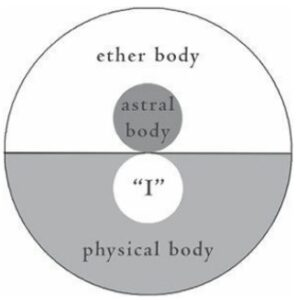
\includegraphics[scale=.5]{a20201211FaithfultoLove-img001.jpg}
\end{wrapfigure}
That leads to the stage of Inspiration. To return to the original idea, Dante started with the image of Beatrice who was not a real woman, or at least not real to him. Nevertheless, that inspired a huge creative output of philosophy and poetry, culminating in his masterpiece.

The final stage is Intuition, when he reaches into the highest heavens. In Intuition, the whole is grasped all-at-one, in its entirety. That is a long way from the physical effects that Beatrice's beauty elicited from him in his youth.

\paragraph{Individuation}

The process of Individuation involves the four primary archetypes: Ego, Shadow, Anima (or Animus), and Self. The intent is not to psychologize the attainments of the initiates. Nevertheless, the journey of the Spirit will have its reflection in the Soul. Therefore, it is helpful to focus on phenomenological experiences, even if, ultimately, they are left behind. That occurs when Inspiration becomes Intuition, that is, the help of sensory images or thoughts are no longer necessary.

The path can be summarized, referring to the diagram on the right (from Valentin Tomberg):

\begin{itemize}
\item \textbf{Ego}: The I of the body, attentive to its needs. What is above the line is unconscious to it. 
\item \textbf{Shadow}: The knowledge of good and evil requires an adversary to push back. Catherine of Emmerich reveals this as an evil being, but not irredeemably evil. 
\item \textbf{Anima}: The unity is broken. A person of the opposite sex reunites. 
\item \textbf{Self}: The return to the Primordial State requires these elements to be integrated in the Self, represented by the circle. 
\end{itemize}
\paragraph{Ego}
As Jung defines it, the Ego

\begin{quotex}
forms the centre of the field of consciousness; and, in so far as this comprises the empirical personality, the ego is the subject of all personal acts of consciousness. 

\end{quotex}
The Ego can arise only through thinking. Descartes' insight — \emph{I think, therefore I am} — is correct. The intellectual soul is tied to the Ego. That is the spirit breathed into man that lights up consciousness; actually, the source of the light is the Holy Spirit. As the diagram shows, the undeveloped Ego is the I of the body. The etheric and astral bodes (vegetative and animal souls) are unconscious to it.

The esoteric student will be encouraged to recall the first time he had the awareness of being an I, i.e., a separate being. The long-term task is to bring the unconscious into awareness. This will develop a stable Self and beyond that, even higher states of being.

\paragraph{Shadow}
\begin{quotex}
The shadow is a moral problem that challenges the whole ego-personality, for no one can become conscious of the shadow without considerable moral effort. To become conscious of it involves recognizing the dark aspects of the personality as present and real. \flright{\emph{Aion}}

\end{quotex}
Young children act spontaneously; there is no separation between emotion and response. Traditionally, there is no moral responsibility until around the age of seven. Thus, in the exoteric tradition, children begin confession at that age; that trains them in the task of becoming conscious of the Shadow.

Yet even that is insufficient. All negative emotions and thoughts, idle fantasies, and the like need to be brought into awareness.

\paragraph{Anima}
This is actually the Syzygy Anima-Animus, but I can only write from the male perspective. The Anima is the most difficult archetype to recognize. Like the physical member that requires a partner to be aroused, so also does the Anima. Mother, Nana, and Sister are the first to contribute to it.

\begin{quotex}
The mother carefully inculcated into him the virtues of faithfulness, devotion, loyalty, so as to protect him from the moral disruption which is the risk of every life adventure. \flright{\emph{Aion}}

\end{quotex}
Nevertheless, to remain at that level is be infantile, so there must be more. The Anima contains the imagoes of Baubo, all his lovers, Divine Wisdom. Baubo returns in the infamous interrogation scene from \emph{Basic Instinct}. She is hardly safe and consistent.

\begin{quotex}
This perilous image of Woman belongs to him; she stands for the loyalty which in the interests of life he must sometimes forgo; she is the much needed compensation for the risks, struggles, sacrifices that all end in disappointment; she is the solace for all the bitterness of life.

And, at the same time, she is the great illusionist, the seductress, who draws him into life with her Maya — and not only into life's reasonable and useful aspects, but into its frightful paradoxes and ambivalences where good and evil, success and ruin, hope and despair, counterbalance one another. Because she is his greatest danger, she demands from a man his greatest, and if he has it in him, she will receive it. \flright{\emph{Aion}}

\end{quotex}
Recall my childhood vision of the cave; the boy could wander about in the world and take risks, certain that he could find comfort and solace on his return. Now that the primal cave no longer exists, that boy needs to build his own cave and find a new source of solace.

Ancient myths, legends, and tales of chivalry portray tales of men having to prove themselves to his potential lover through various tasks, such as feats of bravery, strength, speed. Or perhaps he will praise her beauty and immortalize her in poems and stories. But she needs to be worth the trouble and few are.

The psychological process becomes complicated since it involves a quaternity: the real man and woman, the Anima, and the archetype of the Wise Old Man (or the Animus and archetype of the Chthonic Mother, often represented by Hecate).

That is why, esoterically, the actually existing woman can be a hindrance. The merely psychological level must be transcended. Then higher forces come into play: the Holy Spirit and Divine Sophia or Wisdom. Nay, they are not archetypes, but rather spiritual realities. Psychologically, the Anima is perturbed with “frightful paradoxes and ambivalences”, and other psychic oscillations. The Holy Spirit is the light of consciousness, Wisdom is His reflection in the Anima. When the waters of the Anima are unperturbed, it perfectly reflects the Holy Spirit and something higher can be born.

\paragraph{Self}
Before the Shadow and Anima are integrated into consciousness, the true Self is also unconscious. The Ego believes he is “in charge”, even while he is buffeted by forces that are unknown or unclear to him. As the diagram above shows, the I needs to become master of the unconscious elements of the etheric and astral bodies. Unfortunately, this final stage of integration has its own dangers, so help is often required along the way.

\begin{quotex}
It is of the greatest importance that the ego should be anchored in the world of consciousness and that consciousness should be reinforced by a very precise adaptation. For this, certain virtues like attention, conscientiousness, patience, etc., are of great value on the moral side, just as accurate observation of the symptomatology of the unconscious and objective self-criticism are valuable on the intellectual side. \flright{\emph{Aion}}

\end{quotex}
This psychological Self is still short of the final goal. By transcending the psychological level, higher levels of the Self, with more integration, can be achieved. Ultimately, it leads to life before the Fall, the return to the Primordial State:

\textsc{Et incarnatus est de Spiritu Sancto ex Maria Virgine}.

\begin{quotex}
[The above formula] contains the trinity of the generator above, of the generant below, and the generated—or: the Holy Spirit, the Holy Virgin and the God-Man. It is at the same time the formula of sacred magic in general, because it expresses the mystery of the union of divine will and human will in the element of blood. \flright{\textsc{Valentin Tomberg}, \emph{Meditations on the Tarot}}

\end{quotex}
Esoterically, blood is the physical organ of the human I.

Man is made in the image of God; the Self is the image of Christ in the soul.

\paragraph{Appendix: Polar Beings}
Often the guys will ask how they can get their girlfriends involved in their path. From experience, I don't see how that can be done. If you get along with your gf and she does not oppose your spiritual quest, that is probably a big success.

The esoteric teaching is that many women may be compatible physically but a much smaller number will be a good match for the soul. But there is only one Eve for Adam; she is your polar being. You will meet her once in your life. I suspect most of you have met her already, and are even with her now without fully realizing it. You need to be fully conscious to see it clearly. She may not be a woman “just like you”, or how you think you are; rather, she will be just like your Anima. The more conscious you are of the Anima, the better will you recognize her.

Two souls who fully know each other become, in effect, a single I. This is the highest path.



\flrightit{Posted on 2020-12-11 by Cologero }

\begin{center}* * *\end{center}

\begin{footnotesize}\begin{sffamily}



\texttt{Sibylle on 2020-12-23 at 07:46 said: }

Thank you very much for this article. I do hope it will resonate with many readers. It certainly touched me since from the practical female perspective relationships remain very much stuck due to the lack of response a woman gets from the soul of a man. (And as a result of that even the “remote control” loses its power, which in turn is interpreted as homo-bi-trans-whatever-sexuality whereas it is just a sign of the enormous distance a man put between himself and his body, let alone his soul.)

What if the cave is a cave full of men instead of women because men went into hiding? It seems impossible to find a woman resembling a man's “Anima” if men refuse to leave the cave and allow that space to women. Of course you are talking about a man's perspective and I absolutely understand that men are afraid of women. Especially nowadays with all this obnoxious behaviour by many females.

It really doesn't contribute to a greater depth of a relationship though if men refuse to take care of themselves. The so called risk taking mentioned in this post does not happen anymore. As a result women need to compensate for the lack of respect men show towards themselves which makes any real intimacy impossible, because the active role becomes the woman's role all along, not only when it comes to the level of the psyche. This change of behaviour makes attraction impossible even before the level of the soul is reached. Sexual attraction cannot arise when a woman needs to make up for a man's missing self respect.

We all know the causes for this mess. However – “feminism” could never have happened with the enormous help of many so called intelligent men who could and should have known better. (But as we know: Every vote counts!) It cannot be left to women alone to clean up the mess. We need a hand. There can be no deeper revelation if there is no quest. Rusalka is a necessary first step. It is impossible to submit oneself if there is nothing to submit to. And believe me, the need for submission has never been greater (as mentioned here\footnote{\url{https://www.gornahoor.net/?p=8417}}).

It is something women give with great joy and very freely if there happens to be a receiver. However it is an act that arises from the occasion where it is needed, it can neither be forced nor demanded.

The “right” woman can only be “right” if she is needed. She can only be needed by someone who has left his cave. If you decide to stay in there, she cannot find you.

In this sense remainig faithful to love means remaining faithful to oneself in allowing this self to be known to itself before it can be revealed to others (a woman). When men don't bother about themselves and remain in their caves women become superfluous. It's planet Adam without the need for any sort of Eve. So imagine what it feels like to be a woman on such a planet. Everything a woman does can been accomplished better by a man. Even remaining in the cave. So why do we exist?


\hfill

\texttt{Cologero on 2020-12-23 at 17:27 said: }

The knight Don Manuel de Leon retrieved a glove from a lion's cage at the request of a Lady. He then slapped her for frivolously endangering the live of a knight.


\hfill

\texttt{Sibylle on 2020-12-24 at 08:11 said: }

This slap probably taught the Lady more than a thousand words about the moral implications of her carelessness. Women never understand the effect they have upon men unless they receive their initiating slap. It is rather an act of information than of dominance.

The Lady will surely have remembered that Knight's slap as one of the most caressing moments of her life.


\hfill

\texttt{Santiago on 2022-06-07 at 00:21 said: }

“…she is the solace for all the bitterness of life.

And, at the same time, she is the great illusionist, the seductress, who draws him into life with her Maya…”

Why must the Anima be both `Madonna' and `Whore'. How is it even possible for her to take up such a contradictory existence? In both dreams and real life, women are capable of the most radical transformations. I don't know how it's even possible to be both so enraptured by someone and yet to be made to experience such fear.

“The Anima contains the imagoes of Baubo, all his lovers, Divine Wisdom. Baubo returns in the infamous interrogation scene from Basic Instinct.”

Some lovers moreso than others; some I will never get over. Mainly from the perspective of dreams, the Anima's relationship with time is also worthy of note. Little forgotten details from years ago will be brought up, or I'm given little premonitions related to the upcoming days or weeks. Sometimes the similarities are even undeniable, beyond coincidence. It's like a game to her, and she responds to the interest I take.

And you hit the nail on the head. Every now and then, something analogous to the Basic Instinct scene does occur, but if I take the bait, holy hell does she make me pay for it. FWIW, I'm never allowed beyond that point. It's like a cruel test.

“The psychological process becomes complicated since it involves a quaternity: the real man and woman, the Anima, and the archetype of the Wise Old Man.”

Kind of a technical queston, but who is the `Wise Old Man'. and how is he related to all this?


\hfill


\end{sffamily}\end{footnotesize}

\section{She who must be obeyed}

\begin{quotex}
From my earliest youth to the present time I have been aflame with the most exalted and noble love. My love was extremely difficult to bear: certainly not because of the cruelty of the lady I loved but rather because of the overwhelming passion kindled in my mind by my unrestrained desire which often caused me to suffer more pain than was necessary. \flright{\textsc{Giovanni Boccaccio}, \emph{The Decameron}}

Only loving like a pure madman can you continue along the road. But how many times do you believe you love someone and in reality you love no one, not even yourself? \flright{\emph{Nos: Book of the Resurrection}}

\end{quotex}
\paragraph{The Anima}
At the end of the \emph{Letter I: The Magician}, \textbf{Valentin Tom\-berg} reveals that the Magician represents the man who has attained harmony and equilibrium between the spontaneity of the unconscious and the deliberate action of the Ego (conscious sense of I). This state of consciousness is the Self or Real~I.

This process of individuation proceeds in stages described by Jung. The ultimate synthesis – speaking from the male point of view – is the integration of the Anima archetype, as described in Two Essays on Analytical Psychology. The archetypes are inborn in the psychic makeup, so the Anima is the image of the woman in the man. This is represented in three ways to be described later. But prior to conscious awareness, the Anima is a dark force, erupting into awareness as unexplained moods and other ways.

In meditation, one seeks to bring the I consciousness into the lower parts of being. In particular, there needs to be more awareness of the workings of the psyche or subconscious. There, one will find other beings, i.e., different “I's” or different personalities, each claiming to be the true~I.

Jung's psychological approach is useful for this process, provided the limitations of psychology are understood. This post is concerned with just one part of the process, achieving harmony with the Anima. The first things to note are any unexplained mood changes. Beyond that, there needs to be a deliberate encounter with the Anima. For example, initiating a conversation with Her and writing it down. In our workgroups, this has been effective; sometimes the effort results in a poem. Of course, careful attention to dreams is necessary; big dreams – i.e., those that have more than a personal content – should be logged.

Note that we have not recommended more books to read. We learn most effectively by trial and error. Ultimately, the Hermetic path is quite personal and one law for all would be oppression. One's book comes at the end of the exploration, not before. Tomberg describes the process:

\begin{quotex}
The pure act in itself cannot be grasped; it is only its reflection which tenders it perceptible, comparable and understandable or, in other words, it is by virtue of the reflection that we become conscious of it. The reflection of the pure act produces an inner representation, which becomes retained by the memory; memory becomes the source of communication by means of the spoken word; and the communicated word becomes fixed by means of writing, by producing the book. 

\end{quotex}
Keep that in mind. The Anima is a mystery, and our verbal descriptions are of its inner representation. She cannot be exhausted by our verbosity.

\paragraph{She}
Jung refers to the character in \textbf{Rider Haggard}'s novel \emph{She} — the one who is called “She-who-must-be-obeyed” — as descriptive of the Anima. She is a mana personality, that is, “a being full of some occult and bewitching quality, endowed with magical knowledge and power.” This, Jung claims, is a projection of an unconscious self-knowledge, described this way:

\begin{quotex}
I recognize that there is some psychic factor active in me which eludes my conscious will in the most incredible manner. It can put extraordinary ideas into my head, induce in me unwanted and unwelcome moods and emotions, lead me to astonishing actions for which I can accept no responsibility, upset my relations with other people in a very irritating way, etc. I feel powerless against this fact and, what is worse, I am in love with it, so that all I can do is marvel. 

\end{quotex}
Obviously, a man who has ever fallen so totally in love will recognize parts of himself in that description. But if he then manages to integrate the Anima, he will gain her mana. This will raise him archetypally to the “mighty man”, e.g., a hero, chief, magician, saint, ruler of men and spirits, a friend of God. It is one of those types that particularly interests us, viz:

\begin{quotex}
Actually, it is the figure of the \emph{magician} who attracts the mana to himself, i.e., the autonomous valency of the Anima. 

\end{quotex}
\paragraph{Dante and other Initiatory Texts}
This teaching is certainly not novel. Rene Guenon mentions some European initiatory texts. Foremost among them are \textbf{Dante}'s \emph{Divine Comedy} and the medieval poem, \emph{The Romance of the Rose}. Both of them are focused, in differing ways, on the integration of the Anima.

For Dante, Beatrice was a projection of his Anima, an unreal woman who led him to higher states. Now Dante lived a man's life: he raised a family, he was a warrior in the battles of the time, he was a poet, philosopher, mystic, and initiate in the \emph{Fedeli d'Amore}. Boccaccio claimed Dante's countenance displayed a Saturnine melancholy, not surprising in such a deep thinker.

Hence, his writings were not at all dry abstractions, but were taken from his own life. In his oeuvre as a whole, he describes people, personal events, dreams, impressions, etc. The trend of some Traditional writers to leave out the personal element as something inferior is not necessarily superior.

The Romance of the Rose is an allegorical poem about uniting with the Rose, despite a series of obstacles. Various personages representing, for example, Reason, Genius, Friendship, the Old Woman, offer different opinions on the task. To regard it simply as an entertaining tale of romance would be a mistake.

Guenon also surprisingly mentions \textbf{Boccaccio}'s Decameron and \textbf{Rabelais}'s Gargantua and Pantagruel as other initiatory texts. They may be too ribald for some, but that may be a technique to hide the real meaning from the merely curious.

The main point, then, of all these works is to show how the integration with the Anima is essential on the Hermetic path.

\paragraph{The Blue Rose}
Folk tales often contain hidden wisdom unlike much of modern story telling that is cynical with ideologically inspired lessons. For example, \emph{the Legend of the Blue Rose}\footnote{\url{http://www.marilynkinsella.org/Fabulous\%20Folktales/The\%20Blue_rose.htm}} is one such tale from China. Note how the lesson of the story is opposed to the commonly accepted serpentine wisdom of our time. For example, the gardener's son, in some MGTOW circles, would be mocked as being in the “friend zone”, while the princess is really attracted to some “bad boy” who mistreats her. However, in the folk tale, the princess is psychologically healthier than Western woman today. She recognizes her real Animus and they live a happy life together.

\paragraph{Germanic Women}
\textbf{Tacitus} in \emph{Germania}, sections 18 and 19\footnote{\url{https://www.gutenberg.org/files/7524/7524-h/7524-h.htm}}, describes the Germanic women of his time. Jung uses them as exemplars of this quality:

\begin{quotex}
Woman, with her very dissimilar psychology, is and always has been a source of information about things for which a man has no eyes. She can be his inspiration; her intuitive capacity, often superior to man's, can give him timely warning, and her feeling, always directed towards the personal, can show him ways which his own less personally accented feeling would never have discovered. 

\end{quotex}
Tacitus notes that the matrimonial bond is quite strict among the Germans, with monogamy being the norm. The woman is not the weak link in that relationship; rather she shares fully in their common life:

\begin{quotex}
That the woman may not think herself excused from exertions of fortitude, or exempt from the casualties of war, she is admonished by the very ceremonial of her marriage, that she comes to her husband as a partner in toils and dangers; to suffer and to dare equally with him, in peace and in war: Thus she is to live; thus to die. 

\end{quotex}
The society is based on chastity, with no “seductive spectacles”, adultery is extremely rare and immediately punished. Young couples are expected to be virgins, so marriage is lifelong. They don't try to limit children through birth control, nor through infanticide as in other cultures.

That opposition to divorce, promiscuity, adultery, and birth control was very influential on the Roman church. Even the Greeks allow divorce and have been inconsistent on contraception. Of course, the neo-pagans believe in none of it.

\paragraph{A Modern Life}
The modern world tries to foist on us certain falsehoods presumably based on “science”. One of them is that a man is genetically programmed for promiscuity. The traditional life of the Germanics reveals the lie. A real man protects his wife and children, desiring to keep them safe and secure, psychologically and spiritually, not just physically. The effeminate man seeks pleasure over protection; he is not our model.

\paragraph{Three Appearances of the Anima}
\textbf{Friedrich Schlegel} in his roman a clef \emph{Lucinde}\footnote{See Section \ref{sec:Lucinde} in this book.} describes three appearances of the Anima: as Wife, as Mistress, and as âme-soeur. He recognized those three qualities in his wife Dorothy. That is, their relationship clicked on all three levels: hylic, psychical, and spiritual.

\begin{quotex}
The imago of woman (the soul image) becomes a receptacle for these appearances which is why a man, in his love choice, is strongly tempted to win the woman who best corresponds to his own unconscious femininity—a woman, in short who can unhesitatingly receive the projects of his soul. …it may turn out that the man has married his own worst weakness. 

\end{quotex}
\paragraph{Wife and Mother}
A man's first female relationship is normally with his Mother. This imprints itself in his psyche:

\begin{quotex}
His nearest relations, who exercise immediate influences over him, create in him an image which is only partly a replica of themselves, while its other part is compounded of elements derived from himself. The imago is built up of parental influences plus the specific reactions of the child; it is therefore an image that reflects the object with very considerable qualifications. 

\end{quotex}
As he matures, that shifts, as Jung describes:

\begin{quotex}
In place of the parents, woman now takes up her position as the most immediate environmental influence in the life of the adult man. She becomes his companion. 

\end{quotex}
\paragraph{Sexual Attraction}
The strongest impulse of the Anima is sexual attraction, which erupts into consciousness in various forms. This is exacerbated by the distortions of the psyche resulting from the fall.

The first is our imaginative faculty in the astral body (animal soul) which is given over to sexual fantasies of all types. These occlude the image of the Feminine as Sophia, while debasing her. She just has an instrumental value. Although a healthy relationship will involve visual, auditory, and tactile elements, these are used not for their attractive qualities to another human being, but rather as stimuli for personal pleasuring. So in Dante's case, his fantasy of Beatrice leads him to higher realms, whereas the fantasy of a so-called poet today (as in pop music) would be more suitable to for the Penthouse Letters.

Another distortion occurs even lower, in the etheric body (vegetative soul). A healthy eros will be oriented towards the Beloved. Most often, however, the eros is indiscriminate, and is attracted to women other than the Beloved. Moreover, the eros may even be directed to other objects, as in fetishes, for example. Since the eros is ideally intended for one specific person, artificial stimulation of the eros can be an obstacle to spiritual progress.

\paragraph{Polar Beings and Courtly Love}
Since the psychological is the reflection of something higher, the Anima needs to be understood in her spiritual reality. The story of Adam and Eve reveals this, since Eve is split off from Adam. She is then his spiritual double, the outer representation of his Anima. Although Jung's archetype is to be understood in a universal sense, it is also intensely personal.

With the Fall, this connection has been lost. This is meant in Tomberg's sense of the archetype that manifests itself endlessly both in history and in each individual. The task of the integration of the Anima becomes intertwined with finding one's twin soul or âme-soeur. \textbf{Boris Mouravieff} refers to that couple as Polar Beings. Drawing on Eastern Christian traditions from Mount Athos, he asserts that at the general Resurrection, the human elite will be formed of polar couples. The meeting of the Polar Couple is a new initiation.

There is much esoteric effort required for that to happen. The first stage is the purification of one's own being. If you find that you are consistently entering into toxic relationships, that is likely due to defects in your own psyche, particularly with the Anima. We are not speaking here of so-called good relationships which are mostly a mutual agreement to “settle”, which eliminates the element of risk, yet also prevents the full attainment of something higher.

This was understood much better in the Middle Ages with the ideal of Courtly Love involving the Knight (or Warrior) and the Lady of his Dreams. We have the Troubadours and the \emph{Fedeli d'Amore} as examples. This was Love at the spiritual and objective level, beyond both the carnal and the psychological level.

The Knight and the Lady considered themselves to be spiritually united. Yet they renounced any idea of marriage as such. Typically, the social roles of wife, husband, mother, father were with someone else, not the Polar Being. Moreover, a physical relationship must be avoided as a sacrifice. This is emphatically not some “high-minded” Platonic love devoid of passion. Rather, the physical attraction is quite intense, so its renunciation can be quite painful.

The Knight and the Lady will meet each other once in their lives, but will seldom recognize each other, because they are not ready or have not advanced enough. Sometimes they are given a second chance and that must be obeyed.



\flrightit{Posted on 2018-06-29 by Cologero }

\begin{center}* * *\end{center}

\begin{footnotesize}\begin{sffamily}



\texttt{Therion Exú Rei on 2018-07-23 at 15:40 said: }

the anima is an archetype, archetypes are modes of perception and modes of function. Jung talks about 4 phases of the anima as an mode of perception, how men ig going to perceive the female sex.

they are representaded by eva, helena of troy , maria and sophia.

In the first phase men is under the mother figure, the men in this phase is either a homossexual or a weak heterossexual. That kind of men that is submissive to the female figure. In the second phase the men can see woman as a truly sexual object, but he is under a more of an animal sexuality. In the 3 phase, very rare for modern men, it begins a higher perception, woman is see as a spiritual being, capable of rising men to a spiritual ground. In the fourth phase, is the mysterium conjunctuns!


\hfill

\texttt{Mikkel on 2018-07-28 at 10:52 said: }

If we're talking about the Anima as Jung described I think the article puts out well that “Jung's psychological approach is useful for this process, provided the limitations of psychology are understood.” 

In his talking of phases as you've (Jung?) described, it seems limited and counter to the concept of unity of a principle vs. multiplicity which quickly spirals into talks of “progression”. Perhaps these are not stages that follow from one to another or build on each other, but frames or perceptions of types of men who made them. As psychology is really based on some type of cure or understanding to help change an individual, perhaps we can see that stages or perceptions are different ways of being rather than focused on an individuals perspective? As representational, what do all the figures mentioned represent or say about the spirit that illustrated the feminine with their description as true, perhaps these descriptions of the phases here shows more about the type of spirit and how closely related they are to principle rather than a quality of the feminine being illustrated as truth, albeit the stages described have truth to them, but essentially why do certain people see them that way?


\hfill

\texttt{Michael on 2020-11-04 at 11:12 said: }

Circling back to this…”Typically, the social roles of wife, husband, mother, father were with someone else, not the Polar Being. Moreover, a physical relationship must be avoided as a sacrifice. ”

How does this work with “Schlegel and his wife, Dorothy, turned that common wisdom on its head by incorporating all three aspects into a single relationship.”

Seems like an example of turning common wisdom on its head, but perhaps closer to a synthesis we hear the words of M. (paraphrased) : “All must be sacrificed, but we have not said all must be broken.”


\end{sffamily}\end{footnotesize}

\section{Astray in the Human Jungle}

\begin{quotex}
Turn every negativity to your profit. \flright{\textsc{St John Climacus}}

Courtly love can be effective only if it is based on a Gnosis which is lived, for only a lived Gnosis, on that has been acquired through experience and has gone down into the heart—one joined with Hope that is founded on Faith—will ensure that the knight will have the discernment which will prevent him from going astray in the jungle of purely human reasoning and feelings. \flright{\textsc{Boris Mouravieff}}

\end{quotex}
As we pointed out last time, a consistent theme has been the development of the sense of Self or the Real I. Along with that, we have used the idea of the possibility of using feminine energy as the means for that development. This started, actually, we our first real post on Lucinde by \textbf{Friedrich Schlegel}\footnote{See Section~\ref{sec:Lucinde} in this book.}. The difference between masculine and feminine spirituality should be clear by now. The former, as described by \textbf{Julius Evola} in particular, involves an act of possession of what appears to be a lack, but is really a privation.

The feminine, on the other hand, is more concerned with filling that lack, always in a passive way. Thus, the movement based around a “Law of Attraction” has gained ground in recent years. Its teachers claim that the “universe” will satisfy the lack, presumably in some automatic and predictable way. A recent encounter may serve to illustrate these things more clearly, while providing concrete examples for Evola's and Michelstaedter's abstractions\footnote{\url{https://www.gornahoor.net/?p=7338}}.

\paragraph{Rhetoric and the Feminine Consciousness}
Not so long ago, I heard from a woman — let's call her Erica — who had discovered the Meditations on the Tarot web site. Since she was very interested in that topic, she contacted me to discuss it. She gobbled up all the articles and was full of praise. I gave her the source and she bought the book immediately. After a week of exchanging emails, we agreed to meet for dinner at a posh Palm Beach restaurant.

It would be easy to believe that she had won some sort of genetic lottery. A former internationally known cover girl, she still retained her beauty, and was cultured, elegant, with a sharp intelligence. A true cosmopolitan, she had lived in several different countries. Yet, there was still something deeply sad about her. There was a malaise, bordering on spiritual acedia. She managed to keep it so deeply hidden, I was unable to intuit exactly what it was, given the short time we spoke in person. Nevertheless, she was quite spiritual and claimed to be fully committed to her Catholic faith.

She was a bit intimidated by the Tarot commentary, so she asked me where she could find the “kindergarten” to begin her studies. I assured her that the education she received at her convent school was more than enough kindergarten. Tomberg gives us a deeper understanding of just what she would have learned in her religion classes.

She seemed quite pleased to hear that.

\paragraph{The Feminine Path}
When she began describing her own comparable spiritual undertakings, we could see our differences arise. It should surprise no readers that she had taken an active interested in areas such as the development of psychic powers, angels, crystals, and so on, that is, the whole gamut of the new age. Apparently, there is a college in London that claims to teach such things. Just as in our interview with Aphrodite\footnote{\url{https://www.gornahoor.net/?p=7197}}, she, too, was interested in exotic stones from around the world and their alleged effects on the various chakras.

I mentioned that she was following a very feminine path, whereas Medtarot and Gornahoor are quite masculine. That she agreed with, even pointing out that the men at her psychic studies college were less masculine. The fundamental difference is this: feminine forms are interested in seeking experiences, visions, good feelings, and so on. The masculine paths, on the other hand, are interested in transcending the human condition altogether.

\paragraph{Chakras and the Hero}
Let's look at the chakra studies, for example. Different stones are supposed to correspond to different chakras, which in their turn, correspond to the various endocrine glands. Of course, it is “all good”, and there is no concern about artificially stimulating the lower forces or inadvertently triggering a higher chakra before the person is ready and prepared to deal with those energies.

For example, if the lower chakras represent subconscious or animalistic forces, as \textbf{Carl Jung} says, we are not “honoring the earth” by placing our own selves under their power. Obviously, if everything is “good”, if everything is to be “honored”, then there is no place in this world for the Hero. The Hero knows what is good and evil, what is honorable and dishonorable. Without such distinctions, there is no reason for the quest. That is why the modern mind, in particular, has gone astray in the jungle of purely human reasoning and feelings. And since Christ is the archetype of the Hero, this message is profoundly anti-Christian. Here is Jung, speaking to Miguel Serrano:

\begin{quotex}
Do you know what the Self is for Western man? It is Christ, for Christ is the archetype of the hero, representing man's highest aspiration. All this is very mysterious and at times frightening. 

\end{quotex}
So to the extent that the West loses its faith in Christ, it also denies the Hero. It then denies that man has any high aspirations, since the basest things are now celebrated and honored. All this to avoid the mysterious and the scary. The remaining Knights in the world accept the mysterious and move forward despite the terror.

\paragraph{Chakra Energies}
I'm not denying that such energies exists, just that the stone is not its source. In that system, the I, or Self, is passive. Hence, the stone, or endocrine gland, must be vibrated from the outside in order to produce some effect on the Self. However, the stone represents a privation, a lack of understanding our own psychic centers, so we project our own energies onto the stone. If there is energy blockage in the psychic centers, the better course is to deal with them internally, with the Self as the active force, not to rely on external factors to do that work of self-awareness and self-development for us. This whole line of thought is an example of the lack of self-possession.

In his meeting with Miguel Serrano, Carl Jung offers a deeper commentary on the chakras, which he considers as purely psychic centers of consciousness, not physical entities associated with endocrine glands. He pointed out the interesting point that different cultures may be centered on different chakras, in this sense. As an example, he referred to a discussion with a Pueblo Indian chief, who criticized white people for thinking with their heads. For him, only crazy people think with their heads, and normal people think from their hearts.

A very interesting point that Jung made is that the ancient Greeks also thought with their hearts. This means that it is literally impossible for a contemporary scholar to understand ancient Western culture, to the extent that he is dominated by his head. One must learn, first, to think with one's heart.

Yet, there is something even more appropriate, certainly due to synchronicity. Jung goes on so say this about contemporary Westerners:

\begin{quotex}
They think only with their tongues. They think only with words, with words which today have replaced the Logos. 

\end{quotex}
That may take some time to fully sink in, and is worth an entire article. But basically, he is describing those under the influence of “rhetoric” in Michelstaedter's sense. Rhetoric has now replaced the Logos, through whom all things are created, with an artificial ideology. You see, we are back to the illusions of the causal body\footnote{\url{https://www.gornahoor.net/?p=7224}}, although from a different angle.

\paragraph{Rhetoric and Psychoanalysis}
It is curious that Erica knew nothing of this, although she has been undergoing Jungian analysis for over five years. That can't be cheap, especially since her therapist made house calls. Moreover, she has had another analyst for decades, but can't use him all the time due to his exorbitant rates. She made sure I understood that her analysis was expensive.

However, that is mere rhetoric to me. I was more interested in the process. I asked here the obvious question, “Did she understand the goal of Jungian therapy?” Her immediate confusion showed me that she had never even thought about that at all. Of course, the goal of Jungian analysis is the creation of the Self, beyond the Ego, through the process of individuation.

\paragraph{Magic Weddings}
So I offered to help her through the process of individuation, since great gains can be made in our era through Courtly Love, i.e., a common spiritual journey shared by the Knight and his Lady. For misplaced Knights, born in a place and time where they no longer have a role, this would be their best path. I'm afraid I don't have the requisite degrees or certificates, and I certainly do not overcharge. As I said, there is no acknowledgment of Knights in our day. Now, in therapy, the male role is taken by the psychologist; I don't see how a female therapist, as in her case, can be the catalyst for that process.

Serrano builds on Jung's idea with his own description of the magic wedding. In some ways, he comes close to Tomberg's idea\footnote{\url{https://www.meditationsonthetarot.com/the-word-is-made-flesh}} that the fruit of the union of the male and female principles in consciousness gives birth to the Logos, the Christ within, which Jung claims is the archetype of hero in the West. That is the true self.

While both Jung and Serrano describe this wedding in terms of an alchemist and the mystical sister, a physical female is not absolutely essential from the male perspective.

Man is self-sufficient, since in him the anima is the passive element. To give birth to the True Self, the anima must be pacified so that it can receive the imprint of a higher source. That is why Jung says that a physical woman is not absolutely necessary for the individuation process. Rather, she is a privation, so the energy of the anima exists in the man and can be claimed in an act of self-possession.

The situation is different in a woman. For her the anima is the active element. So to make it the passive element would force her to no longer be a woman, psychically. That is why she needs a man to complete the individuation process, and that role was usually taken up by the analyst.



\flrightit{Posted on 2014-06-09 by Cologero }


\chapter{Metaphysics of Love}
%Dante
\section{Fedele d'Amore and the Tantric Path}

The \emph{Fedele d'Amore} was an initiatic society of Italian poets, and Dante was the most prominent among them. For these poets, the image of the beloved revealed the Divine Sophia, thereby awakening higher stages of consciousness. For Dante, it was Beatrice who served as his guide. 

A similar tradition existed among the Islamic poets. Ibn Arabi had his Nizam, the beautiful and intelligent daughter of a patron. For Hafiz, it was the vision of the beautiful daughter of a nobleman that led to his vocation as poet and mystic. 

Some suspect a direct connection between the Sufis and Dante. However, Dante learned his craft from the Sicilian poets in the court of the Viking Holy Roman Emperor, Frederick II, in Palermo. Since Sicily had previously been ruled by the Arabs, it is not unreasonable to postulate an indirect connection through those Sicilian poets. However, a typological similarity does not necessarily involve an historical connection. 

In an attempt to clarify and justify such a spiritual way, I will list the major ways. 

\paragraph{The Way of the Fakir}
The way of the Fakir involves the use of physical austerities to develop concentration and will. This is continued in certain practices of Christian monks who use painful tourniquets or among Orthodox Jews who wear abrasive underwear. Although certain powers and a strong will can follow from such practices, as the Buddha discovered, they are insufficient to lead to full awakening. 

\paragraph{The Way of the Monk}
The way of the Monk uses devotional practices and rituals to transcend ordinary life. In this way, the emotions can be purified and lower desires transcended. The study of theology can lead to sound doctrine and a steady mind. However, this type of knowing is still at the level of the rational mind or faith, and does not rise to the level of gnosis or Wisdom. 

\paragraph{The Way of the Yogi}
The way of the Yogi is what is most commonly recognized as the ultimate spiritual path. The Yogi transcends all the personal or individual states of being, and may become a \emph{jivan-mukti} — that is, someone enlightened while still in the body. More commonly, such states are not permanent, and usually involve a series of epiphanies that leave an indelible mark on consciousness. The examples of Plotinus and Solovyov come to mind. 

This way is what Guenon describes, and is characteristic of the Brahmin caste. 

\paragraph{The Way of the Knight}
This is the way of someone active in the world, and is characteristic of the Kshatriya , the way favored by Evola. It involves both the development of the intellect and the will. Since all material effects have their origin in spiritual causes, this path requires not only a deep understanding of the world of spirit, but also the power and courage to bring such ideas into manifestation. Furthermore, it is only through the power of the human will that the will of the angels (or gods) can manifest on the plane of human consciousness. 

Although this path involves the whole being, and may be sufficient in itself, since it deals with the action of the world-soul or Sophia, there is often something lacking. That is why the knights of yore took up the practice of courtly love. 

\paragraph{The Way of Tantrika}
This is the most mysterious way, little known until recent times, and subject to many misconceptions. It is usually confused with pure sensuality, whereas its real aim is the development of power through the harnessing of sexual or attractive energies, particularly the power to bring cosmic ideation into material manifestation. 

Often women are attracted to the sensual nature, particularly if they have been introduced to certain tantric practices prematurely. (It is not so important for men.) 

The other manifestation of this way is Sex Magick. However, in practice this devolves to little more than a sexualized way of the Fakir. For example, Aleister Crowley's descriptions of sex magick\footnote{\url{https://www.gornahoor.net/?cat=51}} are hardly appealing and turn out to be little more than tedious sexual gymnastics. Certain powers appropriate to the Fakir may be developed in this way, but it is ultimately self-limiting. 

The true way of Tantrika involves a Knight and a Lady, who participate on the path together. Indications of this are give by Miguel Serrano\footnote{Section \ref{sec:TheTest} in this book.} and Boris Mouravieff in \textbf{Gnosis}. Further elaboration of this topic must await future essays.



\flrightit{Posted on 2010-06-23 by Cologero }

\begin{center}* * *\end{center}

\begin{footnotesize}\begin{sffamily}



\texttt{Will on 2010-06-24 at 12:09 said: }

I agree that Dante used his love for Beatrice as a path to the Divine, but I'm not convinced that the Fedele d'Amore were an initiatic organization. It seems difficult to make that case in regards to Guido Cavalcanti, for example. Do you know of a good source of information about this?

Your point about possible Sufi influence on Dante is well-made. A Spanish author in the 1920s made the case for Dante having effectively `stolen' the work of Ibn Arabi, but I tend to take a more Traditionalist approach that if their insights coincide, it points to a common realization rather than simple borrowing.

It seems to me that the way Dante used his love for Beatrice as a method or technique – a love that was never physically consummated – has a parallel in Plato's descriptions of the erotic ascent, which also involve using the energies of sexual desire and appreciation of beauty to open a path to the Divine. The Phaedrus and Symposium both contain striking descriptions of this.

And by the way, the translation of The Individual and the Becoming of the World is great. Thanks for making it available.


\hfill

\texttt{Will on 2010-06-24 at 18:35 said: }

Do we know that the Fedele d'Amore were an initiatic organization? While it seems clear that Dante used his love for Beatrice as a path to Divine Love, I'm not sure if we can say that Guido Cavalcanti and the other poets were engaged in similar practices. Can you refer me to any good sources on this?

I am struck by the similarity of Dante's method to the one described by Plato in the Phaedrus and Symposium. He also advocates using the energies of sexual desire and appreciation of beauty to open a path to the Divine. I wonder if perhaps the Sufi practices you mention were not influenced by the Platonic tradition. After all, the Muslim world was the keeper of ancient Greek philosophy at this time.

Regardless, I am in agreement that just because Dante and Ibn Arabi and Plato share similar insights, it does not mean there was any direct influence. Rather, it speaks to a common realization, or a kind of `objective metaphysics.'


\hfill

\texttt{Cologero on 2010-06-27 at 11:20 said: }

Are you familiar with “Insights into Christian Esoterism”, where Rene Guenon includes several chapters about the Fedeli d'Amore under the heading of “Some Christian Initiatic Organizations”? There is simply too much information to be summarized in a comment.

In “The Esoterism of Dante”, Guenon writes:

The history of the Hermtic tradition is intimately linked to that of the Orders of Chivalry, and was preserved at the time in question by initiatic organizations such as the \emph{Fede Santa} and the \textbf{Fedeli d'Amore} ,..

You can also look at the reference to Dante in Evola's “The Hermetic Tradition”.

Your insights are good, and you should see the connections between “love”, “eros”, the “woman”, “Wisdom”. Solovyov has similar insights and tried to bring them into the outer church. Even Auguste Comte, in his strange way, stumbled on a rudimentary understanding of this symbolism.


\hfill

\texttt{Will on 2010-06-27 at 20:46 said: }

Thank you. I have read Guenon's book on Dante, but not the other that you mention. I am also largely ignorant of Comte and Solovyov, so I will add them to my list of thinkers to look into.

When I was doing research on Dante a couple years ago, the most helpful sources that I found were The Metaphysics of Dante's Comedy by Christian Moevs, Titus Burckhardt's essay “Because Dante Is Right,” and Henry Corbin's Creative Imagination in the Sufism of Ibn Arabi, in which he has some discussion of Beatrice as a “theophanic” figure.

This is the article that led me to Corbin's work:

\url{http://henrycorbinproject.blogspot.com/2009/02/corbin-dante-i-fedeli-damore.html}

The author of this piece makes similar claims about the Fedele d'Amore, and says that Guido Cavalcanti was their leader. However, when I read Cavalcanti's poetry (albeit in English translation) it seemed to lack the transcendent dimension that so dominates Dante's work.

This, of course, does not mean that he wasn't an initiate or that the Fedeli d'Amore was not an initiatic organization. Perhaps Cavalcanti failed where Dante had succeeded in growing his earthly love up to the heavens. Or perhaps he did not fail, and his realization simply took a different expression which is not as externally religious as Dante's.

I don't pretend to fully understand this method, but from what I can see, I think you are right to compare it to Tantra. Some Buddhist lineages teach a method wherein one views the whole phenomenal world as one's lover. Still other tantric methods involve viewing one's lover as an enlightened being, and thereby practicing `pure view.' The idea, as I understand it, is that when one falls in love, it is due to the enlightened nature shining through, and so one can use that as part of the path, trying to extend the appreciation and pure vision one naturally feels towards the beloved towards all of existence.


\hfill

\texttt{Cologero on 2010-06-27 at 21:17 said: }

There is an excellent book that contains commentary and all of Solovyov's works on Sophia, published as “Divine Sophia” by Judith Kornblatt.

I am not recommending Comte without reservation, as he was somewhat of a strange character. I have a quirky interest in him because he was also a mathematician and for his counter-revolutionary views. He was not a Traditionalist. Nevertheless, I was quite pleased to read a favorable essay about Comte by Solovyov; so there are at least two of us who noticed the same thing about Comte.

For an overview of Comte see here: Auguste Comte\footnote{\url{http://www.gornahoor.net/library/AugusteComte.pdf}}.


\hfill

\texttt{Will on 2010-06-27 at 22:35 said: }

Vladimir Solovyov sounds like a fascinating person. I will check out the book you recommended.

Here is a nice quote from Henry Corbin on this matter:

“In … 1201 when he reached Mecca, the first goal of his pilgrimage, Ibn `Arabi was thirty-six years of age…. He received the hospitality of a noble Iranian family from Ispahan, the head of the house being a shaikh occupying a high post in Mecca. This shaikh had a daughter who combined extraordinary physical beauty with great spiritual wisdom. She was for Ibn `Arabi what Beatrice was to be for Dante; she was and remained for him the earthly manifestation, the theophanic figure, of Sophia aeterna…. For theophanism there is no dilemma, because it is equally far removed from allegorism and literalism; it presupposes the existence of the concrete person, but invests that person with a function which transfigures him, because he is perceived in the light of another world.”

And from Seyyed Hossein Nasr:

“The beauty of woman is, for spiritual man, an unveiling of the beauty of the paradise that he carries at the center of his being … She is the theophany of esotericism and, in certain modes of spirituality, Divine Wisdom … reveals itself to the gnostic as a beautiful woman.”


\hfill


\end{sffamily}\end{footnotesize}

\section{Fedeli d'Amore}

\begin{quotex}
To every heart which the sweet pain doth move,\\
And unto which these words may now be brought\\
For true interpretation and kind thought,\\
Be greeting in our Lord's name, which is Love. \flright{\textsc{Dante}, \textit{from his initiation poem to the Fedeli d'Amore}}

The various `ladies' celebrated by the poets attached to the mysterious organization of the Fedeli d'Amore from Dante, Guido Cavalcante, and their contemporaries to Boccaccio and Petrarch, are not women who actually lived on this earth but are all, under different names, one and the same symbolic `Lady'. who represents transcendent Intelligence or Divine Wisdom. \flright{\textsc{Rene Guenon}, \emph{Insights into Christian a Esoterism}}

\end{quotex}
It was necessary to write a poem in order to be initiated into the Fedeli d'Amore. In 1283, Dante sent the group a poem about a dream he had, asking for an interpretation. In his dream Amor (Love) appeared with Beatrice. He received several responses and was allowed into the group.

\paragraph{Alchemy}
The Divine Comedy can be regarded as an alchemical work, since it describes, the transformation of human matter to the gold. There is this correspondence with the alchemical process:

\begin{itemize}
\item \textbf{Nigredo}: inferno, the fire that burns 
\item \textbf{Albedo}: purgatory, the fire that purifies 
\item \textbf{Rubedo}: heaven, the creative fire of love 
\end{itemize}
There has been speculation about Dante's ties to the Knights Templar. We are not really interested in the conspiracy theories or any external evidence. Rather, for us, what matters is the internal evidence. Esoteric works contain “Easter Eggs”, i.e., unexpected clues that are the key to the deeper meaning.

The obvious connection link is \textbf{Saint Bernard of Clairvaux}, who was both the spiritual director of the Templars and Dante's final guide. Dante chose St Bernard as his final guide to indicate his affinity to the Templars. Before exploring the transformation described by the Fedeli d'Amore, there are some items that may seem speculative initially.

\paragraph{Satanic Trinity}
Satanic trinity is the ape of the Divine Trinity. It is depicted as the three headed Satan. These refer to Lucifer, Mephistopheles or Ahriman, and one unnamed for now.

\paragraph{The Female Trinity}
The other trinity consists of Mary, Lucia, and Beatrice.

Mary is the second Eva. This is also indicated in the Ave, which is the reverse spelling of Eva.

St Lucia is an interesting insertion, since “Lucia” is the anagram of acuil (=acquila), the eagle. \textbf{Valentin Tomberg} deals with the symbolism of the eagle in the Empress card. For example,

\begin{quotex}
The eagle shows the aim of magical power; it is its emblem and its motto, which reads: “Liberation in order to ascend”. Together they represent a magnificent flight; they aim, as a whole and each taken individually, at the ideal of the sublimation of human nature.

“The science of LOVE” is the sceptre of the Empress, which represents the means by which the aim of magic is attained. 

\end{quotex}
Beatrice is the celestial reflection of Dante's first love, and stands for Wisdom.

\paragraph{The Troubadours and the Sicilian School}
Although the ideal of love in spiritual literature is ancient (Song of Songs, for example), the more immediate precursors of the Fedeli d'Amore were the Troubadours of Southern France. They sang of Courtly love, which was based on nobility and chivalry.

Its roots go back to the French Troubadours, whose theme was always courtly love between a Lady and a Knight. Courtly love was [and is?] experienced as erotic attraction mixed with spiritual attainment. However, the relationship was not sexually consummated. Rather, the knight sought the admiration of his Lady through his deeds and accomplishments, often undergoing ordeals at her request.

The same theme was adapted by the Sicilian School\footnote{\url{https://en.wikipedia.org/wiki/Sicilian_School}} under the patronage of Holy Roman Emperor \textbf{Frederick II}. They invented the sonnet form, and an initiate had to write a sonnet in order to be accepted into the school. This spread to the Fedeli d'Amore where Dante perfected the sonnet form.

\paragraph{Polar Beings}
There are three levels of attraction between a man and a woman: carnal, psychic, and courtly or spiritual love. Carnal love, obviously, desire the physical act and nothing more. With psychic love, there is an emotional connection. Traditionally, there has always been a period of engagement before the couple has carnal relations, despite their strong physical attraction.

The deeper the connection, the more creativity is expressed in the relationship. \textbf{Boris Mouravieff} describes this phenomenon:

\begin{quotex}
On all planes, the objective sign of Love's participation is the creative spirit which animates the subjects for whom it has become an aim. Conversely, if we think we are in Love but objectively do not notice an increase in creativity on any plane, either in ourselves or in our partner, we can be sure that the relationship is based on anything but Love. 

\end{quotex}
Tomberg likewise asserts that true creativity cannot exist without love. Emotional bonds may fade, but there is a higher love between polar beings. In this case the commitment is much deeper:

\begin{quotex}
The Knight and the Lady of his dreams, whether they are so in truth or honestly claiming to be so, must endeavour to act in all circumstances of their inner and outer life as if they were already united in their consciousness of the real I, which is indivisible although bipolar, and ONE for their two Personalities and their two bodies. 

\end{quotex}
A Polar couple will meet each other once in their lifetimes, but will seldom recognize each other. The Knight must learn to see the image of his Lady in his consciousness, and vice versa. Even when they do meet, there may still be obstacles. That is due to the deformations in their inner being and different karmic burdens.

\paragraph{Transformation}
Carnal love is connected to the etheric body (vegetative soul) and psychic love to the astral body (animal soul). In the fallen state, these two bodies are under the influence of demonic spirits indifferent to, or even opposed to, human attainment. The etheric body will create images in the astral body, or the astral body may be so overcome with emotion that it does not seek anything higher.

This is the clue to the alchemical transformation. The etheric and astral bodies need to be purified. Eva represents the astral body in the Fall, so the opposite of the Fall is Mary. The goal, then, is the transmutation of the chaotic soul into the pure mirror of the divine word.

For the individual, this will be the development of the Real I. For the polar couple, they will develop the I together.



\flrightit{Posted on 2018-09-16 by Cologero }

%otros
\section{A Theory of Love}

\begin{quotex}
The Temptation of Love is to overwhelm the lovers, to hypnotise them as it were, and reduce them willing or unwilling, to a state of passivity which is actually, in the end, the state they desire. \flright{\textsc{Charles Williams}}

\end{quotex}

In our current age of extremes, in which MGTOW and dogmatic feminism each seems reasonable positions to their proponents, we can forget how previous generations understood the ideal of Romance between men and women.

\paragraph{Charles Williams and Romantic Theology}
The Inkling \textbf{Charles Williams} wrote a thesis that attempted to provide an outline for Romantic Theology, which he regarded as a new branch of the subject. Although he could not find a publisher in his lifetime, it was published about a dozen years ago. The theological part of the book is rather conventional, so is less interesting to me. However, Williams' real skill is in literary criticism. He mentions \textbf{Plato}'s \emph{Symposium} and \emph{Phaedrus} as well as the \emph{Zohar} as valuable to his topic. However, since they are not explicitly Christian, he does not make use of them. Instead, he refers to three “masters” in particular:

\begin{itemize}
\item \textbf{Dante} 
\item \emph{La Morte d'Arthur} by \textbf{Malory} 
\item \textbf{John Donne} 
\end{itemize}
Williams describes Donne as a writer of “love-poetry expressing itself in a religious vocabulary.” Besides Donne, Williams looks at several other poets; however, it would be too distracting to cover them in this piece.

\begin{wrapfigure}{rt}{.3\textwidth}
	\centering
	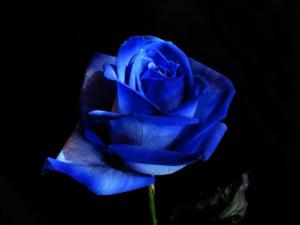
\includegraphics[scale=.3]{a20190131ATheoryofLove-img001.jpg} 
\end{wrapfigure}

Since Williams wrote an influential study of Dante, \emph{The Figure of Beatrice}, it is no surprise to see him as the first Master. Dante, he says, “is the spring of all modern love literature.” Unfortunately, Williams doesn't follow the trail back to the Sicilian poets who influenced Dante, and beyond them, even, to the Troubadours. On the other hand, Dante did it better than his predecessors. He had the ability for deep introspection as well as the ability to express it in words. This is how Dante described his falling in love with Beatrice:

\begin{quotex}
I say that when she appeared from any place, there was no enemy remaining to me, but a flame of caritas possessed me, which made me pardon anyone who had offended me; and if anyone had then asked me concerning anything, my answer would have been only Love, with a face clothed in humility. \flright{\emph{La Vita Nuova}}

\end{quotex}
The story of King Arthur's knights, with the quest for the grail, needs to be unravelled. Williams uses three of the knights to illustrate the different degrees of love.

\begin{itemize}
\item \textbf{Bors}: love in marriage. 
\item \textbf{Percival}: love between two persons who are in contemplation of, but without desire for, each other, their desire being only towards God 
\item \textbf{Galahad}: love whose contemplation and desire is alike towards nothing but God 
\end{itemize}
\paragraph{Three Degrees of Marriage}
\begin{quotex}
There is no accepted agreement upon what the state which our grandfathers used to call `falling in love' involves. It is neither sex appetite pure and simple; not, on the other hand, is it necessarily related to marriage. It is something like a state of adoration. \flright{\textsc{Charles Williams}}

\end{quotex}
I suspect that his grandfathers believed that love led to marriage, but to understand Williams' larger point, we can look at the evolution of the idea of marriage.

\begin{itemize}
\item \textbf{Age of the Father}: Divorce and even polygamy were allowed due to the weakness of the people. 
\item \textbf{Age of the Son}: Marriage is monogamous without the possibility of divorce. Only the death of one of the spouses can end the marriage. The two become one flesh. 
\item \textbf{Age of the Spirit}: Alchemical marriage or the union of souls. The two become one spirit. 
\end{itemize}
\textbf{Baldassare Castiglione} seems to see things more deeply then Williams, when he writes:

\begin{quotex}
Love is defined as desire awakened by beauty, and by progressive illumination passes from sensible beauty to spiritual, and from spiritual beauty to divine: from lust to love, and from love to religion. The duty of the lover is service and honour; the reward of the right lover is intellectual communion with his lady. 

\end{quotex}
The character Jane in one of \textbf{Dumas}' novels says:

\begin{quotex}
Let us forget earth, let us realize heaven; let us share our thoughts, our joys, our griefs, our aspirations, our tears, so that in this unfleshly communion of minds and souls there may be in our eyes pride, in our heart-throbs purity, in our speech chastity, in our consciences calm. 

\end{quotex}
Has your girlfriend ever spoken to you like that? Perhaps the pressures arising from marriage obscure that state of adoration. Finally, here is a thought from Castiglione, that is the very opposite of the Playboy/Charlie Sheen philosophy:

\begin{quotex}
Who does not know that women cleanse our hearts of all evil and low thoughts, of cares, of troubles, and of those heavy dejections that follow in the trains of these? And if we consider well, we shall recognize also, that in respect to the knowledge of high things, so far from turning away men's mind, women rather awaken them. 

\end{quotex}
\paragraph{Francis and Clare}
The relationship between Francis and Clare is an unusual case. It is threatening to clerics and friars who fail to understand it. For example, some see a scandal in the fact the Francis and Clare would sometimes travel together. Hence, they try to downplay the erotic element, even if some moderns can see nothing but the erotic element.

We are embodied beings, so a complete love includes body, soul, and spirit; there is attraction on all three levels of being. In ordinary cases, however, the erotic element takes the form of sexual imagery. Eros then turns inward and demands its satisfaction, thereby preventing its ascent to the spiritual. When the mind is purged of all such sensory images, then eros is turned upwards. Beatrice led Dante to the knowledge of the higher things, yet Dante still experienced his love for her on multiple levels. Williams describes Dante's reaction in terms of the three centres recognised in medieval physiology: the heart, the brain, and the liver.

\begin{itemize}
\item The \textbf{heart}, where the spirit of life dwelled, exclaimed to him: “Behold a god stronger than I, who is to come and rule over me.” 
\item The \textbf{brain} declared: “Now your beatitude has appeared to you”. 
\item The \textbf{liver}, where natural emotions such as sex inhabited, said: “O misery! How I shall be disturbed henceforward!”
\end{itemize}
Yet, the lower emotions can be overcome. Williams describes a different mode.

\begin{quotex}
Virginal love is that which, arising normally between a man and a woman, finds its method in the rejection rather than the acceptance of the ordinary physical approach. It is not particular ascetic: that is, it does not deliberately set aside the graces of the body: it may rather be defined as that kind of love which is so occupied with contemplation that it has no room for desire. 

\end{quotex}
This ideal was \emph{de rigueur} in certain Russian spiritual circles early last century, including Jacques Maritain and his Russian bride Raissa. Perhaps, as saints, Francis and Clare are its perfect embodiment.

\paragraph{Polar Beings}
\begin{quotex}
Nevertheless, neither is the woman without the man, nor man without the woman in the Lord. \flright{\textsc{1 Corinthians 11:11}}

\end{quotex}
Drawing on the Orthodox tradition, \textbf{Boris Mouravieff} describes what the calls “polar beings”. There are three paths to follow, with mastery of the sexual centre a necessary part of the training:

\begin{itemize}
\item \textbf{The monk}: avoids the influences of the world 
\item \textbf{The man in the world}: although the past is difficult, life itself offers more opportunities for spiritual growth. By control of the sexual centre, love can be experienced in the emotional and intellectual parts of the soul. This leads to the realisation of the real I. 
\item \textbf{Polar beings}: a man and a woman working together can produce even more rapid results. However, this requires that they be perfectly compatible for that purpose. They will realise the Real I together, as on. Everyone will meet his or her polar opposite in this life, but will most likely not recognize the other as such. 
\end{itemize}
I will quote Mouravieff extensively without comment, since there is little to add.

\begin{quotationx}
The romance, by which Christian society expressed the principle of reciprocal choice, reached its climax in the Middle Ages. … this romance of tomorrow is called on to cement the indissoluble union between two strictly polar beings, a union which will assure their integration in the bosom of the Absolute.

The vision of such a romance has haunted the highest minds for thousands of years. We find it in platonic love, the basis of the singular romance in the myths of the Androgyne man; of Orpheus and Euridice; of Pygmalion and Galatea… This is the aspiration of the human heart, which cries in secrecy because of its great loneliness. This romance forms the essential aim of esoteric work. Here is that love which will unite man to that being who is unique for him, the Sister-wife, the glory of man, as he will be the glory of God. Having entered into the light of Tabor, no longer two, but one drinking at the fount of true Love, the transfigurer: the conqueror of Death.

This work, done by man and woman working together, can develop with extraordinary power and give rapid results… on condition that from the esoteric point of view the two beings entirely condition that they are a perfect couple, that is, that their combination reservations concerning the peculiarities of their human type — reflects the relation between the absolute `I' and the `You' before the Creation of the Universe.

In centres of culture in the cycle of the Holy Spirit, the love-romance—a feature of the previous Cycle—will give place to the unique love-romance of polar beings, those who will be called upon to shape the society of tomorrow.

In this true Romance, the attitude of the Lady contributes much if not all to the victory of the Knight. Her refined and artistic intuition will understand the meaning of love: that is, to love with all the fibres of one's being, up to integral identification, in a glorious dash towards the same goal.

This return to the perfect unity of polar beings is not given freely. It is the exclusive privilege of those who have crossed, or are ready to cross, the second Threshold of the Way. It is through realization of the totally indivisible unity of their real `I'. by two polar Individualities arrived at the second Birth, that the original sin can and must be redeemed. This is the solution for private and for public life. This is also the peace of the Lord.

A man must begin by a conscious search for his polar being. Polar beings will necessarily meet in life, in certain cases more than once. Only the confused ties contracted in this life by each of them, as a result of their free movements, combined with the karmic consequences of one or more previous experiences, can divert the man or woman from the only being with whom they could form a Microcosmos.

Deeply buried in lies, they do not generally know how to appreciate the gift they are given. Often, they do not even recognize each other. If this is the case, then an agonizing question is put: is there one or more means to detect our polar being, and if so, what are these means? To meet that person, to do so without recognition, to let our polar being pass by, is the worst mistake we could possibly make: because we would remain in our factitious life, without light. Distortions of this kind make it more difficult to recognize the polar being,

It is necessary to permit every being coming into this world to carry within himself the image of the polar being; this image is expressed, in each case, by means of the organ of the opposite sex which exists in every being in a state of non-development.

For man to recognize his polar being, he must be fully attentive on all planes accessible to his consciousness. In fact, as a result of the distortion of the film, the meeting always occurs in circumstances and in a manner least expected, generally at a moment and in a form which resembles nothing he could have ever imagined. The rule enforced is precise: to recognise his polar being, man must know himself. This is obviously logical: to recognize his alter ego, man must first recognize his own ego.

From the first meeting, in the presence of the polar being, both the `I' of the Personality and the `I' of the body vibrate in a manner which resembles nothing felt before. The reason for this is that these `I's find themselves then in the presence of their first love which continues through the centuries. Without clearly being conscious of it, the polar beings know each other; and this knowledge, as ancient as they are themselves, is expressed by the voice of their subconsciousness. This creates an atmosphere of absolute confidence and sincerity from the moment they meet. There is a touchstone here: polar beings do not lie to each other. Soon afterwards, vague reminiscences of past experiences will start to come to the surface in their waking consciousness.

Only an infinitely small minority of human beings feel the anguish caused by their inward isolation and ardently aspire to find the Lady of their dreams. Before one can aspire (to something) one must at least think (about it). This thought must literally devour the Knight's heart, forcing him to accomplish the most perilous feats with the aim of finding the object of his aspirations.

The great mystery lies in the fact that the real I of polar beings is one and indivisible. One for the two of them.

Now we will represent the case of polar beings who are conscious of their polarity and who aspire to royal union: that of the Knight and the Lady of his Thoughts. As a prelude to their complete union this aspiration, after it penetrates into their waking consciousness, will gradually impregnate the I's of their Personalities, thus creating an amorous or courtly love which is quite different from that experienced by the normal run of human beings. This sets their hearts aflame and inspires them with the courage to look for the means which will enable them to overcome all the karmic obstacles that appear on their road.

by the autonomy of his life, every Personality produces a particular Karma. Among other consequences, one result is that two polar beings can be born, not at the same time, as should normally happen, but with a difference in time which in certain cases can be considerable. All this `muddle' explains why polar beings so rarely recognize each other spontaneously at the moment of their encounter.

If a man, burning with a valiant heart, becomes a Knight in order to follow the Fifth Way, he must list for that alone. He must cultivate a double desire:

1. To merit the joy of recognizing in himself the image of his polar being 

2. To merit the joy of recognizing her when they meet 

The general rule, which should be rigorously applied is: to attain the desired goal it is necessary to think of it without ceasing. This is the active concentration that is needed.

Courtly Love is the raison d'etre for the couple of polar beings: for the Knight and the Lady of his Dreams; without it, their polarity remains spiritually sterile and they fall back into the common condition. Its practice, however, demands sacrifices and `exploits'. These are tests. For those who surmount them, the salutary effect of Gnosis is doubled; when it is enriched by experience, theoretical knowledge becomes living knowledge.

In the Middle Ages, the Knight and his Lady, who considered themselves spiritually ONE — in our terminology, polar beings— did not venture into marriage. On the contrary, they parted, accepting the risk of never meeting again and knowing that if they did not triumph over a hard test, their love would degenerate, losing its meaning and its marvellous power. They knew that, by separating from each other for an exploit, they stood the chance, while a premature marriage would be reduced to nothing.

There is no exception to this rule: it applies to all, beginning with the couple of young and just polar beings; and it is even more obligatory between two polar beings who meet at a mature age, when life has already burdened each of them with a karmic load. In such cases, the first sacrifice demanded is the renunciation of a physical relationship, and the first exploit consists in the methodical liquidation of the respective karmic burdens, keeping in mind that the big or small `Gordian knots' which make up these burdens must be untied, not cut.

If the presumed polar beings ardently and effectively undertake some esoteric work in the same direction, useful to the Cause, the moment will come when they will be purified. Having become courtly, their Love will assume all its objective force, and in the purity rediscovered in this way, they will finally be convinced of the reality of a polarity that they had felt intuitively. There is no possibility of error at this stage. At this moment, the Second Birth will unite them forever in the midst of the vivifying Love; and death, finally conquered by this, will lose all semblance of catastrophe for them. 

\end{quotationx}


\flrightit{Posted on 2019-01-31 by Cologero }

\begin{center}* * *\end{center}

\begin{footnotesize}\begin{sffamily}



\texttt{Han Fei on 2019-02-05 at 00:46 said: }

Might I ask the obvious question. Why should lovers avoid physical union? What is wrong with it?

Of course deep down inside some of us may suspect the general direction in which the answer may lie. Among the Romans, there was a seemingly profane custom of keeping a wife, a mistress and a slave. Each woman satisfied one of man's particular needs, for procreation and co-management of the house, another for loving companionship and the last for satisfaction of carnal lusts. When one is in the company of his or her beloved, doesn't the impulse to procreate often fall into the background, at least when our minds are lucid? 

In his lesser known works, J.R.R. Tolkien seems to have touched upon the theme of the polar couple extensively, from his description of Celeborn and Galadriel to the tragic and perilous romance between Beren and Luthien. And of course one can draw a parallel from his own marriage as an impeccable example of such a union.


\hfill

\texttt{33 on 2019-02-06 at 07:52 said: }

There isn't anything `wrong' with it, Han Fei, but what Cologero discusses here is not ordinary marriage. (Of course from the Christian perspective, sexual relationships outside real marriage commitment should be abstained from; why this is so can be explained thoroughly in esoteric.) But in this case we're dealing with a special path. The voluntary renunciation of sexual consummation with a `polar being' here is not due to the `sinfulness' of a legitimate human sexual relationship, but rather one of methodological initiatory expediency: the voluntary renunciation of consummation on that natural bodily plane may serve to intensify realization of the corresponding union on a higher, inner plane. These powerful alchemical energies are directed inwardly instead of being released outwardly. That being said, there are certain tantric traditions, even in Buddhist Vajrayana, that incorporate the energies of union on the physical plane as well in a related form of alchemical romance, attempting to synthesise the higher and the lower union. But for my own part, I tend to believe that the latter path is actually more difficult, and that deliberate renunciation of outer consummation of such polar attraction is more powerful in effectuating the inner realization. This will not be the same in all cases, of course, but the right-handed approach has something very important to teach the contemporary world, with its obsession that `love' must necessarily lead to sexual union, which is its desired end.

By the way, I don't know if Cologero has read what Philip Sherrard has to say on the problem of the sexual relationship in Christianity:

\url{http://www.studiesincomparativereligion.com/public/articles/The\_Sexual\_Relationship\_in\_Christian\_Thought-by\_Philip\_Sherrard.aspx}

Apparently there's also a book titled `Eros and Christianity ' which I have not read.


\hfill

\texttt{Simon on 2020-01-07 at 07:48 said: }

Great article, it inspires me to think about my encounters with women much more deeply. There are two points, both regarding karmic influences, which I could use some further elucidation on, due to my lack of doctrinal knowledge.

1. „Only the confused ties contracted in this life by each of them, as a result of their free movements, combined with the karmic consequences of one or more previous experiences…“

Regarding the „experiences“ mentioned here in the last sentence, do they refer to romantic experiences or to experiences on other planes of being, potentially „before“ this earthly life in which they then play out?

2. „…every Personality produces a particular Karma. Among other consequences, one result is that two polar beings can be born, not at the same time, as should normally happen, but with a difference in time which in certain cases can be considerable.“

If anybody could shed further light on this for me, I would be most thankful. As far as I know (and have read on this site as well), the popular modern conception of reincarnation (i.e. multiple earthly and human incarnations, each carrying karmic load from the preceding ones) is most certainly not in line with Tradition properly so called. If this is so, how am I to properly understand Mouravieff here, that is where do these karmic influences that determine the differential in age come from? From freely chosen actions or thoughts in pre-incarnate existence on another plane?

Thanks in advance and please excuse my naïveté regarding this issue.


\end{sffamily}\end{footnotesize}

\section{David and Bathsheba}

\begin{quotex}
I have found in David, the son of Jesse, a man after my heart, who will do all my will. 

\vspace{-1.5em}

\flright{\textsc{Acts 13:22}}


My flesh and my heart may fail, but God is the strength of my heart and my portion forever. 

\vspace{-1.5em}

\flright{\textsc{Psalm 73:26}}

And David had success in all his undertakings, for the Lord was with him. 

\vspace{-1.5em}

\flright{\textsc{1 Samuel 18:14}}

\end{quotex}
\paragraph{David}
King David is one of the Nine Worthies\footnote{\url{https://www.gornahoor.net/?p=331}} who best represent the Chivalric ideal. As a proto-knight, he engaged in battle, he loved, he had friends and enemies, he sinned, he repented, he cried out to God. He was the King of the Heavenly City on earth and a Prophet of God

That made him a real man in the traditional sense, a man who has actualized all his possibilities. Valentin Tomberg explains:

\begin{quotex}
King David was more human than all men of his time. This is why he was anointed by divine order by the prophet Samuel, and for this reason the Eternal gave him the solemn promise that his throne would be established for ever.

\end{quotex}
In this respect, he is a type of Adam. Adam, as the first man, was also a ruler, having dominion over the earth, plants, and animals. Adam brought wisdom to his kingdom and taught survival skills to the human race.

So David serves as an example, not necessarily for monks or other religious types, but certainly for men active in the world. That is why Ibn Arabi's meditation on the \emph{Wisdom of Existence in the Word of David} emphasizes the Will:

\begin{quotex}
The power of the Will is immense. Nothing occurs in existence nor disappears from it without the Will. 

\end{quotex}
Nothing can thwart God's will. However, man chooses the means, which may either be in opposition or in conformity to the Divine Will.

\begin{quotex}
It is only commanding the means, not the command, which brings things into being. None opposes God at all in what He does in respect to the command of the Will. Opposition only occurs in respect of the command of means. So understand that!

\end{quotex}
If there is anything transgressive in David's behaviour, it was not because he was opposed to God's will; rather, the means may have been inappropriate. However, “All's fair in love and war,” as the saying goes.

\paragraph{The Imaginal Realm}
\begin{quotex}
Changing the appearances of things, walking on water, climbing Mount Qaf, all fall in the category of events that Suhrawardi mentions as taking place in the “intermediate Orient”. In other words, they are psychic events whose scene and action are set in neither the sensible nor the intelligible world, but the intermediate world of the Imaginable, the world of symbol and of typefications, the place of all visionary recitals. it is the world in which spirits are corporealized and bodies spiritualized. \flright{\textsc{Henry Corbin}, \emph{Avicenna and the Visionary Recital}}

\end{quotex}
We are familiar with the metaphysical distinction between the world of the Intellect and the world of the Senses. What is often lost, however, is awareness of the Imaginal realm in between the two. Corbin has done much to recover the ancient interest in the imaginal realm. Each realm is associated with a specific sense:

\begin{itemize}
\item \textbf{The Intellectual Realm} is associated with the sense of hearing, which is the most subtle sense. That is why the highest revelations come from hearing. 
\item \textbf{The Imaginal Realm} is associated with the sense of sight. It is the place of visionary experiences. 
\item \textbf{The Sensual Realm} is associated with the sense of touch, which is the deciding factor in determining the real. Thus, a rainbow is not real, because it can't be touched, even though it can be seen. 
\end{itemize}
Usually the imaginal realm is unconscious, i.e., that part of the world that is not represented in consciousness. As such, there is little or no awareness of its existence. In esoteric training the student is taught how to become aware of the contents of the subconscious. However, if the visions arise spontaneously or unexpectedly, they can be frightening. Corbin develops this idea:

\begin{quotex}
This darkness is ignorance or, more precisely, unconsciousness of ignorance — that is to say the natural man is in a state of ignorance and cannot even be conscious of that state. To free himself from it, he must pass to the darkness; this is a terrifying and painful experience, for it ruins and destroys all the patencies and norms on which the natural man lived and depended — a true “descent into hell”, the hell of the unconscious. That [Suhrawardi] discerned the psychic event, the redoubtable initiation into knowledge in the true sense, into the saving gnosis, is greatly to his credit.

\end{quotex}
When reading a sacred text, we often come upon passages that seem contradictory, impossible, or even scandalous. That is a clue that the text should not be understood at the sensual level. Rather, the images are part of the Imaginal Realm. So the answer is not more historical research or textual analysis. Instead, the reader must look deep within; often the meaning will be found there. Obviously, there is no point in relating random historical events if no deeper meaning can be attached.

The story of David and Bathsheba is like that. On the material level it sounds scandalous. But on the Imaginal level, there may be some deep insights. This story, then, is not just about two historical personages, but about events in your psyche which you can observe.

After all, David and even Bathsheba have been held in high regard, the former as a model of chivalry, as a king, as a prophet, and even a type of Jesus, not just by men but even by God. And Bathsheba has traditionally been considered a type to the Virgin Mary, Sophia, the Queen of Heaven.

So consider this a small meditation on their love story, which can be recreated today in your own consciousness, as a psychic event.

\paragraph{Bathsheba}
David was walking on the roof when he spotted Bathsheba bathing. The roof indicates that David was observing from a higher state of being, the level of the Spirit. After seven wives, and a harem, the sight of yet another naked woman cannot account for David's strong reaction to Bathsheba. Just as Adam recognized in Eve:

\begin{quotex}
She is bone of my bone and flesh of my flesh.

\end{quotex}
David saw in Bathsheba the “soul of his soul”.

Unlike his other wives and concubines, Bathsheba was unique, the woman of destiny with whom he has been entangled for eternity. What he saw was the beauty of his soul. As \textbf{Saint Theresa d'Avila} expressed it:

\begin{quotex}
we shall see that the soul of the just man is a paradise, in which God takes His delight. Nothing can be compared to the great beauty and capabilities of a soul; however keen our intellects may be, they are as unable to comprehend them as to comprehend God.

\end{quotex}
Ordinary men can only see physical beauty. A real man finds true beauty in the soul of a woman. When a man is truly attracted to a woman, he will go to extraordinary lengths to get her attention. That is because the quest for unity is also the quest for God.

She, on the other hand, had to do nothing to attract David's attention. That is why a man's love can be so mystifying to a woman. Sibylle told me\footnote{\url{https://www.gornahoor.net/?p=13757}}:

\begin{quotex}
To a woman the love of a man is incomprehensible. She sees it, she hears it, she might enjoy it, be overwhelmed by it and eventually fall in love, but she does not comprehend it.

\end{quotex}
Does not that incomprehension echo Saint Theresa? If you try to understand love intellectually, you will misunderstand. If you try to judge by human standards, you will misjudge.

David and Bathsheba desired a spiritual marriage. Earthly marriage ends at death, and sometimes mercifully so. Uriah is a symbol of that, because, on earth, we all too soon get wrapped up in relationships that are inappropriate. Hence, Uriah represents Bathsheba's lingering attachment to carnal things, and her bathing is a symbol of her purification.

David must also be purified. To possess Bathsheba, he needs to come to terms with his lust and his jealously of Uriah. Since David's means displeased God, he was convicted of sin by the prophet Nathan. The spiritual child born of that relationship is spiritually dead. David confesses:

\begin{quotex}
I have gone astray like a lost sheep; seek thy servant, for I do not forget thy commandments. \flright{\textsc{Psalm 119:176}}

\end{quotex}
Then David is purified when Nathan forgives his sins. Only then, was a special son, Solomon, born.

\paragraph{Solomon}

\begin{quotex}
She came from the ends of the earth to hear the wisdom of Solomon, and behold, something greater than Solomon is here. \flright{\textsc{Matthew 12:42}}
\end{quotex}

The hieros gamos produces a child of wisdom, the true self. Solomon personifies Wisdom. As such, he is the type of Jesus. Solomon's kingdom prefigures the Kingdom of Christ, the eternal kingdom.

As Solomon's mother, Bathsheba is the type of Mary, the Queen of Heaven. At that time, the mother of the King served as Queen. (Otherwise, which of Solomon's wives would be queen?) So the true offspring of David and Bathsheba is Wisdom, just as Mary's offspring is Jesus. David and Solomon had faults, otherwise revelation would have ended with them.


\hfill



\paragraph{Note on Art} In the Middle Ages, Eve and Bathsheba were the only nudes that could be painted, for obvious reasons. However, I have refrained from including such art in the body of the text to avoid misunderstandings.



\flrightit{Posted on 2021-08-29 by Cologero }

\begin{center}* * *\end{center}

\begin{footnotesize}\begin{sffamily}



\texttt{Tannheuser on 2022-04-05 at 14:29 said: }

It's worth comparing the Bathsheba episode to how David came beforehand to possess his wife Abigail. She too was married to an unworthy husband, Nabal, but David refrained from killing him, and the Lord himself struck Nabal down (1 Samuel 25:38), after which David married Abigail (the mother of the prophet Daniel). In a similar way to how David threw aside his earthly armor and weapons in his fight with Goliath in order to rely purely on the help of the Lord, here we see the same attitude with regard to his courtship of a married woman.


\end{sffamily}\end{footnotesize}

\section{Dreaming the Same Dream}

\begin{quotex}
I don't remember well, and in fact I know nothing absolutely nothing at all, about the women I have loved.

Papan answered: That simply means that you have never loved. You simply have no idea of love as an absolute concept. Loving is knowing. It is also like a crime since it involves death, burial, and resurrection. … Love is something very serious. Today it is completely forgotten.

Love in fact is a strange and secret chemistry, in which the androgynous is born. This is true and complete love; everything else is different. Have you ever noticed how impossible it was to fuse yourself with the person you thought you loved, even though sleeping in the same bed? There is always something separating you, a thread of air, a different dream. Can the lovers be truly united if each one dreams a different dream? If you ever begin to dream the same dreams as your love, then you will be able to create the new star, the star of Him-Her, El-Ella. \flright{\textsc{Miguel Serrano}, \textit{The Ultimate Flower}}

\end{quotex}
The ideas of Tantra Yoga have been capturing the popular imagination, not least of all because of the lascivious interpretations put upon it. But metaphysical writers such as Miguel Serrano\footnote{See Section~\ref{sec:TheTest} in this book.}, Aleister Crowley\footnote{\url{https://www.gornahoor.net/?p=51}}, and Julius Evola have made Tantra Yoga an integral element of their thought. Few are aware that this is also part of Esoteric Christian teaching as revealed by Boris Mouravieff with the idea of Polar Beings. Only Serrano and Mouravieff, however, tie it in with the idea of Love, such that the woman is more that the instrumental means for the man's enlightenment (or pleasure). A discussion of Mouravieff's system will await another time.

\begin{wrapfigure}{rt}{.3\textwidth}
 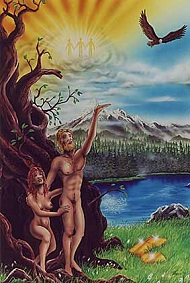
\includegraphics[scale=.7]{a20110608DreamingtheSameDream-img001.jpg} 
\end{wrapfigure}

Serrano was greatly influenced by Jung's idea of the Mysterium Coniunctionis, or the creation of the Androgyne. If every man and woman is a star, the spiritual and inner union of man and woman creates a new star. In a sense the woman surrenders her separate life, living on in the man in his consciousness. As Papan tells him:

\begin{quotex}
All that remains for me therefore is that other road of magical love which will deliver me over to you when I die. In this way I will continue to live, preserved in your memory. Do you realize that in a sense you are a kind of cemetery? You carry so many other around in you, and give them life through your memory of them.

\end{quotex}
By “dreaming the same dream” and sharing visions, the man and women are united. Her salvation comes from him, while she, embodying Wisdom or Sophia, reveals himself:

\begin{quotex}
When I came into her room I no longer spoke, but sat down in a wicker chair beside the window, and silently allowed her visions to pour over me, certain that hers and mine were the same, while all the time she looked through me as though I were a window.

\end{quotex}
Serrano, as a champion of the ascetic-heroic attitude, rejects the physical possession of the beloved:

\begin{quotex}
It should be known then that, in reality, the solution is to be able to bring Her back to life to resurrect Her within his soul.

\end{quotex}
Obviously, this refers back to \textbf{Kalacharaka Tradition} in Tibetan Buddhism. There are three levels of Tantra corresponding to the tripartite nature of man.

\begin{table}[h]\small\centering
\begin{tabular}{rp{17em}l}
\toprule
Karma mudra &
This involves a real female partner, part of the realm of desire. &
Body\\\midrule
Jnana mudra &
At this level, the Yogi creates an image in his imagination. The realm of form. &
Soul\\\midrule
Maha Mudra &
At this level, the Tantrika is formless, with no separate existence. &
Spirit\\\bottomrule
\end{tabular}
\end{table}

Karma mudra (physical woman) and jnana mudra (imaginary woman) are common occurences, available to anyone, with no discernible effect on any sort of gnosis or enlightenment. It is the practice of the Maha Mudra that interests us. In the first two levels, the woman is a privation to the man, while at the third the privation is overcome. The female element is absorbed into the man, creating a being superior to either of them separately.

Sophia, or the Virgin, is the World Process unfolding in our consciousness. As long as the Virgin is objectified, the World Process represents a privation to us, something outside us, beyond our command. It runs on its own. We represent this Process as horizontal, while the action of the Spirit is vertical. The separation and objectification limits the Power of Spirit. The male principle is Spirit (formless), the female principle is the flow of forms revealed in consciousness.

The task of the Yogi is to bring those principles in harmony, to “dream the same dream”. By ascetical and hermetic practices, he quiets the mind, to open a clearing in Being, where Spirit can act. The Virgin then is the perfect reflector of Spirit, revealing to him what He is. In this way, a new child is born\footnote{\url{https://www.meditationsonthetarot.com/the-word-is-made-flesh}}: the Androgyne, the Self, the Christ.



\flrightit{Posted on 2011-06-08 by Cologero }

\begin{center}* * *\end{center}

\begin{footnotesize}\begin{sffamily}



\texttt{Cologero on 2011-06-24 at 22:52 said: }

I found this rather odd story about “dreaming the same dream” in the Rolling Stone hit piece on Michelle Bachmann\footnote{\url{http://www.rollingstone.com/politics/news/michele-bachmanns-holy-war-20110622?page=3}}:

\begin{quotex}
Bachmann claimed that back in her college days, she was up one night praying with a female friend of hers when “the Lord gave each one of us the same, exact vision… It was a picture of me, marrying this man, in the valley where his parents have a farm in western Wisconsin.” Meanwhile, miles away, Marcus “was repairing a fence on the farm where he worked, and the Lord showed him in a vision that he was supposed to marry me.”

\end{quotex}
Leaving aside the unappealing content of her neo-Christianity, Bachmann illustrates the remnants of an archaic consciousness in the modern world: visions, communications with a god, destiny, and the obsession with the ties of family and religion. In contrast, the author represents the post-modern mind and there is, apparently, no point of contact between the two. Instead of an objective and dispassionate essay, he resorts to hysteria, a quality unbecoming in a man. For “those who know”, however, this is just another battle between fideists and post-modernists and is viewed dfferennntly. The post-modernist rejects every aspect of the archaic consciousness, while the fideist claims to hold a monopoly of every preternatual and supernatural manifestation in that consciousness.


\end{sffamily}\end{footnotesize}

\section{Absolute Man, Absolute Woman}

In the chapter “Man and Woman” in Revolt against the Modern World, \textbf{Julius Evola} establishes the proper relationship between the two principles. The feminine force is centrifugal with its tendency to chaos, but when aligned the masculine stability, a synthesis results. Thus, the masculine principle must become more fully itself, while the feminine becomes aligned with the masculine. Evola mentions the symbolism of the “bride” in this regard, just as \textbf{Ananda Coomaraswamy} points out that the king is the bride in relation to the purohita.

Evola points out that birth is not by chance. Hence, the being who is a man or a woman must reflect a spiritual difference. This differs from the modern view which sees one's birth sex as something arbitrary, and now, given new medical technology, as even a matter of choice. However, traditionally, a man must fulfill himself as a man and a woman as a woman.

For a man, according to Evola, the highest ways belong to the Ascetic and the Warrior, corresponding to the Brahmin and Kshatriya castes respectively. Both these paths “affirm themselves in a life that is beyond life”, the former through jnana yoga, or total detachment, and the latter through bhakti yoga, or pure action. The woman, on the other hand, fulfills herself as Lover or as Mother. Note, here, that in Evola's scheme the man can fulfill himself totally on his own, but a woman only in relation to a man. Through devotion to her lover or her son, a woman gives herself totally to another being, thereby fulfilling herself. Evola concludes this discussion:

\begin{quotex}
To realize oneself in an ever more decisive way along these two distinct and unmistakable directions, limiting in the woman everything that is man and in man everything that is woman, approaching the absolute man and the absolute woman – such is the traditional law for the sexes, according to the various planes of life. 

\end{quotex}
Perhaps Evola did not exhaust all the roles since men can also be Fathers and some women are ascetics. Logically, it is necessary for men to be Fathers otherwise women could not be fulfilled as mothers. Even among the Kshatriyas, there is the archetype of the Judge who decides with perfect justice. The vaishyas are neglected, but there are many who through dedication to knowledge or service to the community can find fulfillment.

To return to the spectrum of the absolute man and woman, we are left wondering. For example, where do the Ascetic and Warrior sit on this spectrum? Guenon answers this question when he points out that the Brahmin is oriented to superhuman states while the Kshatriya (warrior) tends to the realization of all the possibilities of the human state. This makes it clear that the Ascetic is more transcendent than the Warrior.

\paragraph{The Absolute Man}
What then is the archetype of the absolute man? Evola alludes to it at the beginning of the chapter when he mentions the purusha and prakriti, the yang and the yin. But \textbf{Alexander Jacob} in \emph{A Reconstruction of the Solar Cosmology of the Indo-Europeans} confirms it. He writes:

\begin{quotex}
The formation of the deity as Purusha/Vishnu, the Ideal Man, is the result of the promptings of the divine heart or spirit. This ideal Man is however actually androgynous. 

\end{quotex}
Thus Purusha is the Ideal or Absolute Man, which is clear once the masculine principle is fully understood. Moreover, a man approaches to this Ideal not by eliminating the feminine principle but rather by uniting with it in the \emph{Mysterium Coniunctionis} or Spiritual Marriage. To transcend all lower states is the non-dual state, as the Purusha is also Atman.

A clue to this state is given by the warrior who actualizes all the possibilities of the human state. Or stated differently, he manifests in matter all his latent possibilities; this requires the cooperation of the feminine principle and especially the domination of it. A fortiori, the jnani actualizes all the possibilities of all the states so there is no longer duality between essence and existence. This defines precisely, in the West, God, for whom essence and existence are one.

\paragraph{The Absolute Woman}
If Purusha is the absolute man, then Prakriti is the absolute woman. Prakriti alone is chaotic, undifferentiated, formless, and blind. As such, Prakriti can never be manifested as it is a metaphysical impossibility. Prakriti must be informed by the masculine principle in order to be anything in particular. But Evola had just pointed out that the woman is fulfilled by her relationship to a man, so the Absolute Woman is not Prakriti separate from all influences of the male principle, but rather the woman who is in the perfect relationship to the higher male principle. In other words, she participates in the same Spiritual Marriage mentioned above.

\paragraph{Excursus on German Idealism}
To make these principles real, they demonstrate how German philosophy of the 18th and 19th centuries fed the process of the feminization of the West. When Kant attempted to show that the pure reason was incapable of any knowledge, the result was the abandonment of the male principle. The pure reason, or intellect, is the tool of contemplation. Only the practical reason, or action, could lead to knowledge of God, freedom, and immortality. This is equivalent to raising the feminine principle to the peak.

Those who followed Kant realized the consequences of his philosophy and concluded that the Will was the fundamental principle of the world. Schopenhauer did this quite thoroughly and consistently. In his system, the Will is fundamental, but if the will is not guided by the pure reason, it must therefore be arbitrary, blind, illogical, purposeless, and directionless. Nevertheless, there had to be something more, the Platonic ideas, to give form to the world. However, apparently the will was not directed by the ideas. Because of this Schopenhauer's philosophy provides many interesting insights. Had he raised the ideas above the will, he would have come closer to a real metaphysics. At least he understood the Will to be transcendent to the world.

Nietzsche borrowed Schopenhauer's concept of Will and gave it a direction, the Will to Power. He also dropped the ideas and regarded the world of appearances, all superficial, i.e., not as appearances of anything transcendental. The Will to Power, as a particular manifestation of Shakti, is feminine, and the denial of transcendence eliminates the masculine element totally from his system.



\flrightit{Posted on 2013-02-06 by Cologero }

\begin{center}* * *\end{center}

\begin{footnotesize}\begin{sffamily}



\texttt{Jason-Adam on 2013-02-07 at 14:55 said: }

Wow. This article destroys the foundations of the New Right and pseudo-traditionalist movement based on German idealism entirely.

Philosophically, we need to get back to knowledge of God through as Aquinas taught us.


\hfill

\texttt{Mihai on 2013-02-08 at 03:24 said: }

This should also make clear to the enthusiasts who put Nietzsche's philosophy on the same level with traditional ideas, that there is nothing traditional about his worldview, quite the contrary. He is much closer to a Marx than to a Guenon and even Evola.


\hfill

\texttt{Jason-Adam on 2013-02-08 at 15:01 said: }

The famous Protocols of the Learned Elders of Zion, which Evola considered worthy of reading, classify Nietzsche along with Marx and Darwin as agents of subversion.

Also, the Abbe Barruel reported that Kant was a member of the Illuminati. When taken together, the facts show that German Idealism was devised as a means of destroying traditional Catholic Europe.


\hfill

\texttt{Cologero on 2013-02-09 at 06:45 said: }

If this has any merit: the real history of white Europeans\footnote{\url{http://vimeo.com/48152436}}, it would explain why Western history has been dominated by the kshatriya mentality and why true intellectuality has been difficult to establish. German idealism is a philosophy compatible with the kshatriya spirit.


\hfill

\texttt{Janus on 2013-02-10 at 23:56 said: }

I don't think the new right claims to be based on German idealism, though Evola certainly was influenced by it in his early years.

I wonder about the possibilities for initiation or illumination for women, in this case. I have always wondered whether the masculine and feminine are really limited in the hardline way Evola prescribes. For example, he goes so far in this chapter of Revolt to suggest that while the woman must love the man, the man does not return this love (I'd cite directly but I don't have my copy on hand…perhaps someone knows the passage?), or else risks losing his pure masculinity. Among Traditionalists, I think Charles Upton at least would find problems with this. Tradition in Europe seemed to encourage love given by both parties (and Evola notes this, but seems to think it a deviation of sorts). 

Moreover, I find it interesting that it seems like this suggests that the masculine and feminine only “really” exist in the man, whereas the woman in her pure femininity must submit herself to this. Thus, it seems like while the man is ascending toward his “true Self”, the woman has no Self outside of that of the man. Perhaps this could be more clearly explained and corrected? It seems to me more likely that the masculine and feminine manifest themselves in different ways in different people, surely. We may look at St. Joan of Arc, who clearly manifested a more masculine principle akin to the kshatriya. than any feminine role. I have also heard a similar explanation of those cases where relations happen between those of the same sex; there usually seems to be a “masculine” vs “feminine” role, so perhaps these principles may be harmonized even when it does not appear to be the case on the profane or physical level (this is, of course, the exception, not the rule). Even the sacrament of marriage can be viewed in this light as the masculine and feminine being completed in complementary beings, the man and wife, thus manifesting the Divine unity.


\hfill

\texttt{Paulo on 2014-11-16 at 11:44 said: }

Janus

“I wonder about the possibilities for initiation or illumination for women, in this case. I have always wondered whether the masculine and feminine are really limited in the hardline way Evola prescribes. For example, he goes so far in this chapter of Revolt to suggest that while the woman must love the man, the man does not return this love (I'd cite directly but I don't have my copy on hand…perhaps someone knows the passage?), or else risks losing his pure masculinity.” 

You dont get the point her,the love of men toward women is not the love of dependence,the love of using women as a lifeline,of the repruduction of the same dependece a baby have toward his mother.He gives consciousness love.

“Moreover, I find it interesting that it seems like this suggests that the masculine and feminine only “really” exist in the man, whereas the woman in her pure femininity must submit herself to this. Thus, it seems like while the man is ascending toward his “true Self”, the woman has no Self outside of that of the man. Perhaps this could be more clearly explained and corrected?”

Being women the passive element,she must receive the masculine princible in her self.When men is fully,that is,had aquire the true masculiny,then he can”fecundate”women!

” It seems to me more likely that the masculine and feminine manifest themselves in different ways in different people, surely. We may look at St. Joan of Arc, who clearly manifested a more masculine principle akin to the kshatriya. than any feminine role”

Even in her case,she had visions of swords coming from the sky,had seen visions,a clearly feminine mode of function.


\hfill

\texttt{Hank on 2017-02-28 at 18:25 said: }

Ibn Ashir said « Purity is thine through water which naught else hath changed »

On this, Shaykh al-Alawi said, « Purity is reached through Absolute Water, the Water of the Unseen, that is, the Limpidity which is variegated in Its manifestation, One with Itself in Its seeming multiplicity, Self-manifested, Hidden through the intensity of its manifestation, Absolute in Its relativity––this is the Water which is free from any taint and which availeth for purification; and of It one fo the Gnostics said: `With the Water of the Unseen make thine ablution

If thou hast the secret and if not, with earth or stone.' 

This is the Water of the Unseen which avileth for purification, and all other water in relation unto it is as dry sand, not to be used except when this Water hath been lost.»

tr. by Martin Lings


\end{sffamily}\end{footnotesize}

\section{Man, Woman, and Self}

In \textbf{Emmanuel Swedenborg}'s interpretation of Genesis, Eve appears as the “self” of Adam. The male principle is the Intelligence and the female principle symbolizes the Will. The Will is the “nucleus, the inmost heart of the human being.” The True Will, then, is man's true self …

How then does a man know his true Self, which is not something that can be observed directly, as one of the objects in the world? \textbf{E. F. Schumacher} outlined the four fields of knowledge\footnote{\url{https://www.gornahoor.net/?p=507}}. So, if I cannot adequately answer the question “Who am I”, then there is the question, “Who do you say I am?” A person usually deludes himself about who he is, whereas others easily see through his pretenses.

\begin{wrapfigure}{rt}{.3\textwidth}\centering
 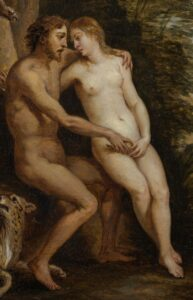
\includegraphics[scale=.7]{a20120908ManWomanandSelf-img001.jpg} 
 \caption{Adam And Eve In Paradise}
\end{wrapfigure}

If Swedenborg is providing the esoteric interpretation, the exoteric understanding is not precluded; to the contrary, it is necessary. For Adam, the Self is dead, represented by the rib since the bones are the last to decay. That rib is vivified by Eve, who appears therefore as the \emph{exteriorization} of his own Self. She is almost his identical twin, genetically the same apart from her having two X chromosomes, his “reciprocal”. Hence, she is the perfect woman for him. In knowing Eve, Adam is knowing himself.

Every woman desires a man who “gets” her, that is, someone who understands her in a deep way. The converse is not identical. A woman, too, wants to know her man, but not always just in his actuality, but also in his potentiality. This often comes across as a desire to change him, leading to a degree of conflict. If this conflict subsides, it indicates she has decided to “settle”, as they put it. On the other hand, it may impel the man to exceed himself. In \textit{Gnosis}\footnote{\url{https://www.gornahoor.net/library/mouravieff3.pdf}}, \textbf{Boris Mouravieff} provides, as examples, \textbf{Wagner} and \textbf{Goethe} who achieved great moments of creativity, inspired by infatuations with younger women.

Sometimes, even among the Medievalists, a woman is represented as an imperfect man. However, that is putting her on the wrong scale, as there do exist imperfect men on the scale whose peak is the Absolute Male. A woman can only be represented on the corresponding scale with the Absolute Female at its peak.

This is a difficult teaching. If the woman is the perfect helpmeet for a man, why is it not always experienced that way? In a relationship, a man is, in some deep way, confronting his own self. To the degree that he lacks self-awareness, the less he sees that. Mouravieff writes:

\begin{quotex}
just as one particular woman produces a different effect of carnal attraction on different types of men, so, on the psychic plane, the creative spirit of a man produces a different psycho-sexual attraction on different women. 

\end{quotex}
The complexities of attraction must be understood on the three levels: carnal, psychic, and spiritual. So called “success” at the carnal level can be mastered if desired. An intelligent man can make changes to himself as he learns to master himself. However, although that is celebrated in the modern world, it is not likely the best use of one's inner resources. Often, a man will entangle himself in harmful karmic relationships that become difficult to extract himself from.

The lower a man is on the scale of the Absolute Male, there is less and less differentiation. Hence, the woman attracted by such a man is likely to be very much like him. At the lowest levels, the lack of differentiation may even appear as an attraction to the same gender. There is little challenge in this case and hence less possibility of achieving self-knowledge.

The higher on the scale, then, the woman will also be correspondingly higher, thereby deviating more and more from each other. That is, ultimately the Absolute Man will attract the Absolute Female, and their respective qualities will be quite different from each other. This hardly means that things go so smoothly, as the higher stages of self-realization get more difficult. In one incident, \textbf{Dante} passed Beatrice and two of her friends on a street in Florence. When she snubbed him, he was so upset he hid in an alley and cried for hours.

Yet Beatrice was the one who prayed for Dante on his journey to Paradise, and became his ultimate guide to the Supreme Identity. Scholars today still debate the identity of Beatrice. But Gornahoor readers now know exactly who she is.


\hfill

For further reading, see Swedenborg and Esoteric Islam by Henry Corbin.



\flrightit{Posted on 2012-09-08 by Cologero }

\begin{center}* * *\end{center}

\begin{footnotesize}\begin{sffamily}



\texttt{O on 2016-12-09 at 20:45 said: }

If the Absolute Man is the same as the sexually differentiated Adam prior to the fall from the centre of the human state, what happens if the spiritual reintegration goes deeper still, becoming the Primordial Androgynous Man? Can we still speak of the Absolute Man if it doesn't have Absolute Woman as its opposite pole, precisely because both poles are reintegrated into the principle preceding them? What is the reaction of the Absolute Woman to a being having realised that state, integrated his opposite and hence become completely free of desire?


\hfill

\texttt{Cologero on 2016-12-11 at 10:45 said: }

@O, I don't think we want to understand “Absolute Man” in such biological terms. Rather, it is the union of the Intelligence and the Will, the head and the heart. Such as we are, the Will and the Intellect are not united, they are usually at war with each other. It is as though we have multiple selves. In Hermetic terms, this union is the alchemical marriage: the Holy Spirit (intelligence) is reflected in the soul (will) giving birth to the Christ, or Logos, as the true self.


\hfill

\texttt{O on 2016-12-11 at 20:29 said: }

That is succinctly put, Cologero, and I agree. But the article differentiates between `Absolute Man' and `Absolute Woman'. which of course is well known from Evola. That is a `sexual' distinction on an archetypal level, but not necessarily a biological phenomenon as known in our existential state. (I think it was C.S. Lewis who wrote somewhere that `gender' differentiation in beings is manifested in modes more essential than biological sex.) What you now explained seems to be different from the notion of an Absolute Man having as his opposite an externally manifested/embodied Absolute Woman, which would be a dual and complementary relation.


\hfill

\texttt{Cologero on 2016-12-11 at 21:33 said: }

@O, rather than repeat myself, perhaps you could comment on this: Absolute Man, Absolute Woman.

Aren't Yin and Yang the ultimate distinction? I believe that the Tao, then, is the union. The Chinese translate the word “Logos” by “Tao”.


\hfill

\texttt{Max on 2019-09-09 at 14:12 said: }

Swedenborg also treats the subject of Polar Beings in his book “Conjugal Love”. So far, I have only had time to eye through it rather briefly, and there seems to be both agreements and some differences when compared to Mouravieff's teaching. From memory, Swedenborg maintains that the prospective polar beings will increasingly polarize according to their efforts, and gradually adapt to one another. There is a potential polarity which is only effectively realised through the sacrament of marriage and conjugal love. In other words, the perfectly polar couple is most likely not found in some sort of “state of nature”. First of all they must crucially be able to recognize one another, which is heavily stressed by Mouraieff.


\end{sffamily}\end{footnotesize}

\section{Journey through the Planets}

\begin{quotex}
All things are in pairs, each the opposite of the other, but nothing the Lord made is incomplete. Everything completes the goodness of something else. Could anyone ever see enough of this splendor? \flright{\textsc{Sirach 42:24-25}}

\end{quotex}
\paragraph{Quantum Entanglements}
Two quantum physical particles are entangled when their states are not independent of each other. That is, if the quantum state of one particle changes, then the corresponding state of the other also changes. This happens instantaneously, even at a distance.

By the Law of Correspondences, two beings can also be entangled. \textbf{Henry Corbin}, in \emph{The Man of Light in Iranian Sufism}, develops this idea from traditional sources. He describes the entanglement this way:

\begin{quotex}
To speak of the polar dimension as the transcendent dimension of the earthly individuality is to point out that it includes a counterpart, a heavenly “partner”, and that its total structure is that of a bi-unity, a unus-ambo. This unus-ambo can be taken as an alternation of the first and second person, as forming a dialogic unity thanks to the identity of their essence and yet without confusion of persons.

\end{quotex}
That implies that every being in the human state has a counterpart. They share the same essence, yet they are different persons. Their “alteration”, although it takes place as conversation, is more like a mirror. The orientations differ, yet they are intertwined: a change in once results in an immediate and corresponding change in the other; hence they share an essential nature. Yet neither one alone is the “real” being. Rather, the two together form a unity, i.e., the true Self.

\paragraph{Adam and Eve}
In \emph{Swedenborg and Esoteric Islam}, Corbin brings this concept closer to home based on revelations to Emmanuel Swedenborg. Analogous to Paul's description of the pneumatic, psychical, and hylic persons, Swedenborg identifies them based on one's own understanding of selfhood or ipseity:

\begin{itemize}
\item The \textbf{Material person} believes that his own self is everything, so his existence would cease without it. This situation is infernal. 
\item The \textbf{Spiritual person} understands, but only in a theoretical way, that the power of thinking and acting arise from his Principle. 
\item The \textbf{Celestial person} has the actual experience of his Self. This Self is like that of an angel. 
\end{itemize}
Adam, in the state of deep sleep, believes that he lives, thinks, speaks, and acts from himself alone. Spinoza, for example, recognized the illusion of that state, although he lacked an adequate solution. Adam rouses from sleep as he sees the illusory aspect of his belief. Fully awakened, he sees that he is no longer alone. Corbin emphasizes the importance of this insight:

\begin{quotex}
it is one of the most profound arcana that there is to meditate upon.

\end{quotex}
Before this transformation, Adam's proprium, or inmost self, appears to the angels as something bony and inanimate. The ribs surround the heart.

Afterwards, Adam's proprium is vivified. Eve is Adam's proprium or Self. Corbin elaborates on this symbolism:

\begin{quotex}
the masculine or man symbolizes the intelligence and everything that relates to it, consequently all tings of wisdom and faith, while the feminine or woman signifies or symbolizes the will, consequently all things relating to love, and consequently relating to life, since life proceeds only from love.

\end{quotex}
Hence, this will is the nucleus or inmost heart of the human being. Thus, the heart is not the nous as some believe, but rather resides in the emotional center. While Eve is the proprium of the internal man, the projection of Eve as other than Adam results in a process of exteriorization. Adam is no longer simply material, but he is not yet celestial. Although he realizes that he is incomplete, he cannot recognize his Self interiorly. Hence, Eve is a projection onto a different person.

Eve, on the other hand, longs for the wholeness that Adam fails to see.

\paragraph{The Double}
The idea of the Double has been part of Tradition, even if the understanding is not always complete. \textbf{Charles Stang}, in \emph{Our Divine Double}, documents the history of this idea. He distinguishes the double into horizontal and vertical versions. The horizontal double appears in pagan stories as well as more contemporary writers. This double is uncanny and even menacing. Rudolf Steiner saw that double in terms of lower beings named Lucifer and Ahriman.

The vertical, or divine, double, on the other hand, was known to Plato. The divine double makes possible the ascent to the Intelligible reality of the divine forms. In the Phaedo, Socrates suggests that the Lover and the Beloved should serve as mirrors to each other. Each sees the best version of himself in that mirror. That does not mean that “Love is Blind,” but rather just the opposite. Love sees what is True and Beautiful in the other, beyond merely material forms.

\paragraph{The Vertical Ascent}
Dante saw the full significance of the Divine Double. On the Earth, our essences are hidden from each other because of the interference of our physical bodies. The outside can conceal the inside. Specifically, our facial expressions and gestures can hide our true thoughts and feelings as much as they might also reveal those thoughts. Hence, Beatrice did not recognize Dante in this life as her double or polar being.

The vertical assent through the planetary spheres represents the attainment of higher states of being. Here, the polar couple help each other; they see in the other what could not be seen. If the gross body veils the truth, then each planet lifts another veil until all is revealed.

Jacob Boehme reveals that Adam was originally separated from Sophia, his feminine Self. In compensation, Eve, the external feminine, was given to Adam. Corbin explains this:

\begin{quotex}
Adam-Eve is the sophianic couple, because Eve is the proprium of Adam, his proprium vivified by the Divine Presence; the Adam-Eve couple has the perception of all the Good of love and the Truth of fa ith and consequently possesses all wisdom and all intelligence in ineffable joy.

\end{quotex}
The polar couple experiences such joy as they journey through the planets. There is no hurry, they have eternity on their side, leading ultimately to the alchemical marriage.



\flrightit{Posted on 2021-05-16 by Cologero }

\begin{center}* * *\end{center}

\begin{footnotesize}\begin{sffamily}



\texttt{Hugo Smith on 2021-05-17 at 22:35 said: }

In the alchemical marriage, shouldn't the two halves be temperamental opposites, since they are incomplete on their own?


\hfill

\texttt{Cologero on 2021-05-17 at 23:31 said: }

temperamental opposites? You are restricting yourself to the psychological plane, not the metaphysical plane. Mirror images are opposite in a way. Next time, try to quote the text where your concern is properly addressed.


\hfill

\texttt{Hugo Smith on 2021-05-19 at 03:12 said: }

Sorry, I was actually searching for the right word there and settled on “temperamental”. The part of the text that gave me pause was “…Socrates suggests that the Lover and the Beloved should serve as mirrors to each other”.

Like you said, this doesn't necessarily imply that the lover and beloved aren't opposites. I was thinking of the Hermetic idea that the lovers must reconcile themselves in each other, like extremes meeting in a sort of spiritual paradox (passive/active, red king/white queen, sun/moon etc).


\hfill

\texttt{Cologero on 2021-05-19 at 07:45 said: }

Do you understand at all how to have a conversation? You don' get a mulligan, i.e., a second chance to make the same point. Consider this from \textbf{Rumi}:

\begin{quotex}\scriptsize\itshape
Listen to the story told by the reed, of being separated.\\
“Since I was cut from the reedbed,\\
I have made this crying sound.\\
Anyone apart from someone he loves\\
understands what I say.” 

\end{quotex}
Do you feel that? Have you experienced that separation from your Beloved? Have you longed to unite? Then you might understand the point.

Of do you wake up every morning, thinking: “I'd really like to reconcile the spiritual paradox today.” We are talking about persons, not abstractions.

\emph{Start taking your life seriously.}


\hfill

\texttt{Hugo Smith on 2021-05-19 at 12:43 said: }

Did I write something that made you mad?

In conversation, people often rephrase things when they think someone doesn't understand.

I'll try to take that last sentence to heart.


\hfill

\texttt{Cologero on 2021-05-23 at 18:35 said: }

No, I don't get “mad”, I am just a good actor. Trust me, I do understand.


\end{sffamily}\end{footnotesize}

%Parece que hay otro de Diotima, anterior
\section{Diotima Unveiled}

As I have been seeking inspiration for a personal project this week, my muse suggested this addendum to the discussion of Diotima. She can not only see past, present, and future, but she can lift souls out of the depths of ignorance and darkness.

The idea of Absolute Beauty is timeless. Hence, one does not ascend the ladder in successive, well demarcated steps. Each step can be associated with a state of being and Guenon explains its meaning.

\begin{quotex}
All states of the being, considered under their primary aspect, abide in perfect simultaneousness in the eternal now. 

\end{quotex}
Hence, one abides on all the steps of the ladder simultaneously. The step you are “on” is just the one to which you direct conscious attention. The most common state is to be in a dream-like state of semi wakefulness, and will therefore, unconsciously, be drawn to the most material step of the ladder, which is physical love.

\paragraph{Sweet Love}
Unlike blasphemy, murder, theft, perjury and so on, which are intrinsically evil, physical love is in itself not evil in itself. However, it may be situationally evil, or perhaps better said, it may be expressed in appropriate or inappropriate ways. That is why such lovers are in the first, or the least painful, level of hell.

Such love is quite delightful which is why it also serves as a trap. Even when it grows sour, as it often does, the being tries to “fix” it or else find it again with someone else. A being on this step is reluctant to move on to higher stages.

\paragraph{Soul Love}
The first stage is restricted to the two lower sheaths of the subtle body: desire and emotional connections. The creative power of sexual energy is restricted to procreation. Obviously, children are necessary for the nation and the family to perpetuate and thrive. There is human love for nation, family, and children, although even animals care for their offspring. To do less, is to live even below the animals. For the ancient Romans, the \emph{proletariat} were those who had nothing to offer society other than their children. So, it is not yet the fulfilment of all human possibilities.

\begin{wrapfigure}{rt}{.35\textwidth}
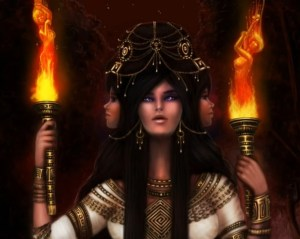
\includegraphics[scale=.4]{a20210216DiotimaUnveiled-img001.jpg} 
\end{wrapfigure}

This requires the training of the emotions to feel a wider range of emotions and to experience them more deeply. And what is distinctly human is intellectual development: the ability to distinguish right from wrong, the real from the unreal. It is the seat of creativity, innovation, and so on.

The more one actualizes his intellectual soul, the more he will be able to recognize those qualities in another. His intellectual life becomes so fascinating and pleasurable, the memories of sweet love begin to fade. Instead, he longs for a higher connection. His desire is to share ideas on music, literature, poetry, history, metaphysics, and the like. Procreation reappears as intellectual creation at this stage.

Sweet love follows a pattern of exhaustion and replenishment; energy is dissipated in its act. Soul love is not like that. It is energizing, energy doubles, so nothing is lost.

When the opportunity is presented, it is taken.

\paragraph{Possession}
It must again be emphasized that this has nothing to do with evolution, or psychological growth. All the stages exist simultaneously; the limitations of human language make it sound like some sort of progress.

A fortiori, soul love is not a substitute for failures at a lower level. If there is no desire at the physical level, there can be no desire, not in its full expression, at the intellectual level. And many men today lack such desire.

Since the present age is a deviation from previous eras, what follows my not follow current trends exactly.

In the past, love and marriage was an option reserved for the lower classes. High status people often had to marry for other reasons, particularly to strengthen political or commercial alliances. For them, the purpose of sex was to create children.

Man tends to want to enjoy before possessing while woman needs to possess before enjoying. This was necessary when women needed a stable relationship in which to raise children and to be protected from strangers intent on enjoying. So the high status woman was secure in her possession but love had to be found elsewhere.

Hence, the notion of courtly love arose. The wandering knight became suitable for that purpose. He is able to enjoy, but he is not in a position to possess because of his wanderings. The early knights were purely physical brutes tied to a particular area, but the solo knight errant developed a code of chivalry and high culture. Thus, the knight could fulfil the soul needs of the high status woman without thereby threatening her marriage or children.

\paragraph{The Veil}
There is a misconception about the veil, as though its sole purpose is to control woman; this is used by Westerners to belittle cultures that still practice it. In more ancient times, pagan and even Christian cultures used the veil. However, it was restricted to high status women. It is a sign that she is more than just a beauty that can be put on display willy nilly for just anyone to see.

The custom persisted until a few generations ago. On more formal occasions, my mother wore a light veil that covered her entire face. Even today a bride wears such a veil at her wedding.

In our time, we can use imaginary veils. Keep that thought as a reminder to try to pierce the veil to see the soul life of the other. If you need some other motivation, that is a necessary Hermetic exercise.



\flrightit{Posted on 2021-02-16 by Cologero }

\begin{center}* * *\end{center}

\begin{footnotesize}\begin{sffamily}



\texttt{Tannheuser on 2021-02-17 at 17:51 said: }

The difference between “sweet love” and “soul love” can also be characterized a difference between passivity and activity. Sweet love (“I am in love”) begins as a passion, something that happens to you, whereas soul love (“I love”) is really an action, or something you do – it requires focus, effort, and engages the higher faculties of the soul. As you say, however, the active and passive exist simultaneously and are interdependent.


\hfill

\texttt{Tannheuser on 2021-02-18 at 13:18 said: }

As for the lack of desire and eroticism on a physical level, Yukio Mishima described this condition as resulting from a lack of contact with the Absolute, or God. It takes only a little reflection to realize the truth of this – it is the only thing separating human eroticism from that of animals mating on a Discovery Channel documentary.

From an interview shortly before his death:

“The beauty-eroticism-death diagram, to which I referred a little while ago, is a concept that demands that the second element, eroticism, cannot exist except in the realm of the absolute. As for Europe, eroticism is only found in the world of Catholicism. This religion has severe commandments whose violation constitutes sin. And the sinner, whether he likes it or not, must appear before God. Well, eroticism is the method of establishing contact with divinity through sin… In the relativism of today's world, however, eroticism is no more than a kind of free sex. It's not opposed to anything. It is sex without any relation to the absolute. In my opinion, nothing could be further from true eroticism.

…In my opinion, one should only speak of eroticism when the human being risks his life and seeks pleasure until death, which is as if he arrived at the absolute from the reverse. If the gods did not exist, they would have to be reborn. And without God there is no eroticism. And because of this way of thinking of mine, I have done the impossible to make the absolute reborn. That is when eroticism arises. What does all this have to do with everyday sex? Well, nothing. Let's say it is a kind of `paneroticism'.

That's it. This search is the main objective of my literature.”


\hfill

\texttt{Paulo Adolpho Zeymer Netto on 2021-02-19 at 03:09 said: }

“The âme soeur (literally “soul sister”) is not just another life partner, and certainly not a concubine. The idea of “sister” should indicate that it is a chaste, not sexual, relationship. Moreover, it indicates a close bond of affinity, not in the biological or genetic sense, but certainly in terms of spiritual races.”

Cologero,please clarify this to me,i have found her,but i could never fell sexual desire for her,so how exactly can we finally be together???What exactly,can bind us together for real and for ever,in a physical sense?


\hfill

\texttt{Cologero on 2021-02-21 at 09:39 said: }

You are an astute reader, Paulo, as I had forgotten that passage. If you look back, one of our very first posts, that has set the trajectory all these years, was about that complete relationship that you desire.

But pay attention to the idea expressed that all the states exist simultaneously, so it is not either/or. It depends on where your consciousness is focused. At one time, you desire her sexually. That is how you experience her for yourself.

Yet, at another time, you will see your kindred soul in her, and relate that non-sexual way. Then you will see here as she is in-herself and for-herself, as a thinking, feeling, willing being complementary to you.

I wish you all the best.


\end{sffamily}\end{footnotesize}


\chapter{Visions of Love}
\section{Leaving the Cave}


In his science fiction short story “The Crime and the Glory of Commander Suzdal”, former Pentagon official and expert on psychological warfare Cordwainer Smith describes a planet which is toxic to femininity. Colonists from earth survive by making their women male. As a result of this modification the colonists start developing a massive hate for normal women and families back on earth and aim for their destruction.

\paragraph{The Need for Intimacy}
“Feminism” has never been about anything feminine. Neither is the invention of the term “toxic masculinity” aimed at men. Both expressions are meant to conceal femininity. They create a narrative which makes it impossible to achieve any kind of consistency between what you really see and feel and what you are supposed to see and feel according to that narrative. As a consequence, men went into hiding and women became male, which in turn rendered femininity an unknown mystery to both men and women.

\begin{wrapfigure}{rt}{.3\textwidth}
\centering
 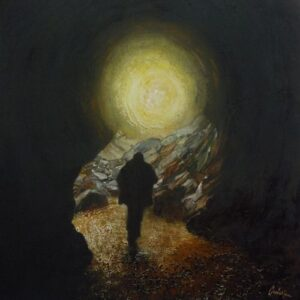
\includegraphics[scale=.75]{a20210113LeavingtheCave-img001.jpg}
\end{wrapfigure}

However, most women on planet Earth are still women and many of them would like to develop more intimacy in their relationships with men. We cannot do this however if deep within their souls men remain detached not only from their wives or girlfriends but even from themselves. Femininity is incapable of making a decision. It cannot become an end in itself — it is searching for a purpose. Intimacy then arises from the feeling of being needed. A man's indifference towards himself makes it impossible for a woman to feel needed as a lover, let alone as a resemblance of his Anima. She will never be able to make up for a man's missing self-respect, because she is thriving on that man's Self. She will cherish, inspire and even submit to it, but she cannot create it.

\paragraph{Integrity vs. Potential}
\begin{quotex}
It is foolish to judge woman with the values of the absolute man even in cases where, by doing violence to her own self, she makes a show of following those values and even sincerely believes that she is following them. \flright{\textsc{Julius Evola}, \emph{The Metaphysics of Sex}}

\end{quotex}
The question is, why should a quality be viewed as a flaw? This development has led to so many misunderstandings, anger, and sadness for men and women alike that it is almost impossible to take a step back and have a look at where we came from. When Weininger bemoans a woman's “lack of being” or Evola explains that for a woman a lie never “breaks her own existential law”, it might seem well and rationally explained from a male perspective, but still contains a judgement or rather a measurement. A woman never draws a border like that. In fact, she cannot.

Potential is to woman what integrity is to man. Potential is boundless and needs to be actualised. There have been many such concepts mentioned on this site, e.g., Purusha and Prakriti, Hyle and Morphe etc. In order to understand a woman's sudden change of opinion, mood, preferences and her simultaneous vacuous conformity to so-called public opinion it is helpful to leave judgement aside for a moment and ask why should somebody want to be like that? Without principles? Without imagination? Is it a conscious choice to be like that? Is it a choice at all? Why should something exist that morphs into something else the moment it feels needed? Without bothering that it is contradicting itself or behaving seemingly disloyal to earlier promises?

There are many disappointed mothers out there who take great pleasure in sharing little anecdotes about how the character of their daughters has undergone a sudden change since their wedding day. Not only did these daughters pick up the vocabulary of their spouses, but all of a sudden also preferred different food, changed their denomination, or even their religion altogether — the list of “changes“ those mothers are keen to spot in their estranged married daughters is endless. Likewise, you will hear complaints from ex-boyfriends and ex-husbands who are perplexed when they realise that their former lovers or wives are finally dressing the way they had always begged them to dress or engage in exactly the kind of sexual practices they had always dreamed of — but they do it now with their new man and would have never done so for their ex-boyfriends or ex-husbands.

So again, why would anyone want to be like that? What is the reason for such a behaviour or is it really simply weakness? Are men not better off without women? No risks, no strings attached?

\paragraph{Authority and Submission}
Of course a woman understands the difference between truth and a lie. She even expects to be told the truth and detects a lie faster than any man would be able to, simply because he does not expect to be lied to. So why does she not feel affected by her own lies whereas a man gets the feeling of utter destruction when faced with a lie? If the mode of existence for women is potentiality this means there is no real lie, no right nor wrong unless a certain potential has been realised.

This realisation is something women cannot do by themselves. I agree, this sounds strange after more than a century during which we have been told that women can do just whatever they want. Maybe we can — if we know what we want. But what we want changes ceaselessly unless there is a real call for submission. However, the following act of submission needs to be received by someone. So why do men tend to run away from that gift? Live up to it! That's exactly what a woman's potential is all about: It is a gift to a man's quest for integrity.

As Nietzsche describes the quest for Sophia in \emph{Thus spoke Zarathustra}:

\begin{quotex}
Brave, untroubled, mocking, violent — that is how wisdom wants us to be: she is a woman and never loves anyone but a warrior. 

\end{quotex}
Male integrity needs to be proven in the same way female potentiality needs to remain opaque, uncategorised and uncharacterised. If a woman is constantly forced into the act of deciding and determining, sexual attraction becomes impossible. A man that does not even bother to take care of himself can't expect a woman to decide what his life is all about.

Women are not capable of creating a man. He has to make the effort to know himself before he can reveal that Self to a woman in order to \emph{know her}. What women can do is to create themselves according to the information they receive from a man. It is an expression of gratitude and not a sign of weakness due to a “lack of being” on the part of the woman as Weininger put it. It is the essence of femininity. What follows actually comes close to what has been termed “Authority” on this blog. It is a natural acknowledgement of the risks a man went through to encounter his own Self.

If this quality of femininity is deemed unnecessary, weak or even a flaw, women become superfluous. Where there is no need for femininity, women deteriorate into a state of always remaining the lesser part, insufficient strange creatures who “lack being” and will be measured according to the values of men, which is probably the reason why, perceiving themselves as lesser men, women have a hard time living up to their own expectations.

Nowadays harm is caused not so much anymore by propaganda which is so obviously nonsensical, but by refusing to see what is right there in front of you. Men and women haven't changed. Words and terms can't create reality. However, perception and acknowledgement of what actually exists influence the way we deal with that reality. That's a challenge men face as well as women. Why not try and work this out together? Leaving the cave\footnote{\url{https://www.gornahoor.net/?p=13522}} and opening up that space for women again would be a first step.

In the science fiction story Commander Suzdal managed to save femininity on earth from destruction by the male-females from the space colony. Subsequently he was stripped of his rank and his name. He was denied life as well as death for not asking for permission to act the way he did. Smith writes: “But the crime was that he had succeeded.” — The same goes for his glory.



\flrightit{Posted on 2021-01-03 by Sibylle }

\begin{center}* * *\end{center}

\begin{footnotesize}\begin{sffamily}



\texttt{Solphomeron on 2021-01-08 at 22:42 said: }

“Body of a woman, white hills, white thighs,

you look like a world, lying in surrender.

My rough peasant's body digs in you

and makes the son leap from the depth of the earth.

I was lone like a tunnel. The birds fled from me,

and night swamped me with its crushing invasion.

To survive myself I forged you like a weapon,

like an arrow in my bow, a stone in my sling. …”


\hfill

\texttt{Sibylle on 2021-01-09 at 17:15 said: }

“I am asham'd that women are so simple

To offer war where they should kneel for peace;

Or seek for rule, supremacy, and sway,

When they are bound to serve, love, and obey.

Why are our bodies soft and weak and smooth,

Unapt to toil and trouble in the world,

But that our soft conditions and our hearts

Should well agree with our external parts?”


\end{sffamily}\end{footnotesize}

\section{Nigredo, Albedo and Rubedo}
\label{sec:NigredoAlbedoandRubedo}

Imagine the life of a contemporary version of “Snow White”. The Evil Queen still wants to kill her stepdaughter. But she has learned from her previous mistakes and got the seven dwarves to abandon their mine. Instead, they are roaming the lands of World of Warcraft, because the Queen made them regard their hard labour as an unnecessary relict from some dark, uncivilised past. For reasons of animal welfare, the hunter was banned from hunting and moved away. So what about the Prince? He is nowhere to be found. Rumour has it that he probably never existed in the first place and had only been designed as a distraction to prevent young girls from becoming astrophysicists and CEOs. By removing every male character from the fairy tale, will the Evil Queen finally achieve the death of Snow White?

\paragraph{The Killing of Snow White}
Nobel Laureate Elfriede Jelinek makes short work of Snow White in her drama \emph{Death and the Maiden I}: her hunter shoots Snow White dead. Needless to say, this act of violence is celebrated as a feminist victory over the so-called patriarchal stereotype of beauty and the feminine wish to please. Snow White is dead and women are no longer perceived as beautiful “objects”. If this assertion were to be correct, it would mean that the only force responsible for the “eternal enslavement” of woman is woman herself. So doing away with her is the way out then?

\begin{wrapfigure}{rt}{.3\textwidth}
\centering
 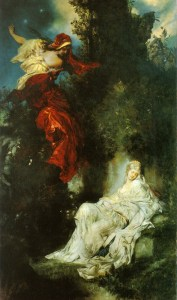
\includegraphics[scale=.6]{a20210127NigredoAlbedoandRubedo-img001.jpg} 
\end{wrapfigure}

In her collection of plays called \emph{Princess dramas}, Jelinek alleges that woman is excluded from truth, because she is incapable of knowing herself as a “subject”. She further states: “[My] texts are partly very philosophic, they make fun of the philosophy of Heidegger, because the areas where woman has been excluded the most have always been thinking and music.” In other words: killing Snow White wasn't enough for Jelinek, she also wishes to exclude woman from Western heritage by negating the very point of music and thinking — i.e., the inclusion of woman into the hearts and minds of men.

In defence of Jelinek one could argue that she might not have had much of a choice other than to kill her inner Snow White in order to survive the harassment by her own mother. If faced with the envy of an Evil Queen and no male rescuers at hand, what is Snow White supposed to do if she wants to stay alive? So before condemning Jelinek for her brutality one has to acknowledge that the death of Snow White could have been her last resort. If the feature that constitutes Snow White's existence is a crime, she simply cannot exist. Matriarchy means the extinction of Snow White as well as the Prince — that is to say: the extinction of love.

\paragraph{Transformation}
\begin{quotex}
But I have no time for such things; and the reason, my friend, is this. I am still unable, as the Delphic inscription orders, to know myself; and it really seems to be ridiculous to look into other things before I have understood that. \flright{\textsc{Plato}, \emph{Phaedrus}}

\end{quotex}
The list of psychological analyses of Snow White is long, rumours about a Rosicrucian origin of the symbolism are widespread — I am not going to recount them here. I would rather like to dismiss the superficial notion that the story is merely about a mother-daughter conflict which will be resolved once Snow White grows up, ceases to be an object of pleasure and finally gets hold of the keys to her own “subjectivity“. The impossibility of being Snow White arises from the Evil Queen's desire for subjectivity. She cannot tolerate beauty that has no intention of its own. Snow White does not suffer from a lack of subjectivity. Under the tyranny of the Evil Queen she is nothing but subjectivity. Without men to marvel at her beauty, to turn her into an object, to save her from death and no dwarves to take care of, she will never be able to “transform” — and fulfil the destiny of the fairy tale.

I am really no expert on alchemy, but in order to achieve “transformation“ you need to do something to a substance. If Snow White is supposed to transform from “nigredo” to “albedo “ to “rubedo“, she needs an impulse from the outside. There is no way for her to develop, if she cannot experience herself as an object. However, it is certainly not the Evil Queen who will bring that change about: her poisoned “gifts” are only meant to encourage vanity and tie Snow White ever closer to her matriarchic rule of total subjectivity.

What possibilities does Snow White have without the hunter, the dwarves and the Prince? How is she supposed to relate to the world if nobody relates to her? There is simply no Snow White left to write a fairy tale about. Without the “transformation” of the subject into an object — dialectic — there would be no “fourth kind of madness” in \emph{Phaedrus}, no pity with Francesca da Rimini in Dante's \emph{Commedia}, no path to any kind of knowledge beyond personal emotions and opinions.

\paragraph{Marcela}
Maybe the “post-structuralist” writer Jelinek sincerely believes subjects have a story of their own. But wasn't it Jelinek's compatriot Wittgenstein who showed that the “thinking, imagining subject” does not exist? That the “I” as a subject remains unattainable for thought because it constitutes “a border of the world”? By killing Snow White Jelinek excluded herself — and as a sophist who is trying to justify her action by claiming the status of a victim, she remains the Evil Queen's most submissive slave.

Now that Snow White has accepted the fact that there will be no hunter, no dwarves and certainly no Prince, she can either become like her tormented and jealous (step)mother or a “sexually emancipated” (Jelinek's self-description), mentally mutilated writer who tries to avoid death by killing herself. So far so good. Maybe there is a third option. Instead of getting bruised by struggling against Wittgenstein's border she could ask Marcela for asylum and accept her own existence without being either ashamed of or sorry for it. Dialectic and devotion can be powerful tools to reduce subjectivity. If she tries really hard, Snow White might manage to transform from “nigredo” to “albedo”. “Rubedo” however will remain out of reach until the Prince finally hears what heaven wills, realises what fate ordains and does his job.

I suppose some would say “rubedo” is dispensable. Those are the ones that tell you the Prince is merely a fantasy and Snow White needs to be killed in order for women to become “subjects”. If “red” were dispensable, Phaedrus would remain without Socrates' second speech and we would know nothing of the “fourth kind of madness”. Some say Marcela represents that fourth kind of madness. Really? Others frame her as the first feminist. Think again: Marcela is the absolute object, completely void of subjectivity and will — thus the negation of the Evil Queen. What the Evil Queen, and Jelinek, fail to grasp, Marcela articulates unmistakably:

\begin{quotex}
until now Heaven has not ordained that I love. And to think that I shall love of my own accord [amar por elección] is to think the impossible. \flright{\textsc{Cervantes}, \emph{Don Quixote}}

\end{quotex}
Love is not a choice. Either you love or you don't, but it is not a decision. You can decide to pursue a relationship with someone. It is a choice to sleep with somebody. You can choose to get married. But to love is not a choice. The choice a woman has to make though is to let go of herself — let go of “subjectivity”. Otherwise she will not recognise love even if a man is on his knees begging for her love. So yes: Snow White actually has to die, not as a victim of the Queen but as a sacrifice to the Prince.

To a woman the love of a man is incomprehensible. She sees it, she hears it, she might enjoy it, be overwhelmed by it and eventually fall in love, but she does not comprehend it. So Marcela is cruel? Is it cruel not to be able to love “of your own accord”? To be unable to feel love unless a man makes you feel it? Why else would music exist? Poetry and art? Are they dispensable? Objects are thought of, written and sung about. Unlike subjects, they are never excluded.


\hfill

The meaning of the alchemical stages are:

\begin{itemize}
\item \textbf{Nigredo}: spiritual death 
\item \textbf{Albedo}: purification 
\item \textbf{Rubedo}: the attainment of a coherent sense of self 
\end{itemize}

\flrightit{Posted on 2021-01-27 by Sibylle }

\section{The Test}\label{sec:TheTest}

Although Evola always writes in a discursive style, he advises us that it is only the rishis, the seers, the clairvoyants who can fully understand. In many ways, Miguel Serrano picks up on some of Evola's themes, though from the perspective of a clairvoyant rather than a metaphysician. In the following passage, Serrano describes the highest Tantric teachings while bringing in the major elements of the esoteric teachings from the Middle Ages: the Grail legends, the Templars, troubadours.

The ultimate end is identical for both Evola and Serrano. Both reject the mysticism of pantheism which looks to the annihilation of the Self and its merging into the Totality. Rather, they proclaim the Absolute Self, the raising up from the merely human to the higher states, the process of deification, atman=brahman.

\begin{quotationx}
Thus were completed the different stages of this most ancient Hyperborean Initiation of A-Mor, revealed in the mystery of the Grail, in the esotericism of the troubadours and the Minnesänger of the High Middle Ages. Transported to the icy wastes of the south of the world, with Parsifal, in a Templars' ship, with the Vermilion Cross on its white sails and all its lights on, as the saga tells us, and from `whence it never returned'. To the true Kingdom of Hyperborea of the White Gods of America-Albania. 

\emph{And while the ultimate test of this initiation was taking place in that ancient night, with a man and a woman lying naked side by side, separated by a sword, without taking possession of each other's physical body, she explained to him in her musical voice full of longing for eternity}: `The light doesn't come from the east. Light is only truly light in the depths of midnight. Now is the depths of midnight. The followers of Lucifer, of the Morning Star, do not beg to be allowed into heaven. They demand to be, because they feel that they have done everything possible to merit being deified. At the end of our road, no fusion with a god or redeemer awaits us. Our way is not the way of ecstasy of the saints but the way of separation of the magicians, of the White Gods who have become absorbed into the sources of creative energy. Creating worlds, loving each other inside and outside eternity. We do not beg, like the lunar troubadour: “Take us back to where you took us from!” We are going to try and change God, giving him a face. Therefore, my love, do not take possession of my body. Let us not create children of the flesh. I will make you pregnant with the son of death. And we will both remain virgins.'

`I understand,' he whispered. `The chastity of the sacred warrior is the nobility of his sexual act, the refusal to tolerate all that is brutal, because his feeling for the beauty of that act prevents him doing so. The Wounded King also said this.'

`It is an immaterial irrevocability. The Grail doesn't tolerate unbridled passions, it loves pious reticence, a reverent attitude. And I will not destroy your magic virility, dividing your flesh and mine, giving you children of the flesh to bring new opportunities to other individuals, when such a great possibility already exists for us. I will not lure you into loving my body in the only way known to the dark age, because that way death will swallow you up. I will never be the Great devouring Mother, the Primordial Female, who will turn you into a vanquished warrior, living in a dream of unfulfilled glories. I will be the She who leads you to heaven. Because it is your magic virility which will enable us to travel along the river of death. Your sacred virility will enable us to return to life. Do you remember the words of the ascetic of the Grail?: “You will become a woman if you love the body of a woman.” This is so: because \emph{only by becoming effeminate could you satisfy the erotic sensibilities of a woman's physical body}. The chaste warrior is the more virile one. To take physical possession of the beloved is to lose one's soul. True possession is the mental possession of all the other bodies. With the memory or your beloved in your heart, you will achieve the Grail. \emph{The genuine orgasm isn't a physical one but another which is endless, and which is produced by your contact with my invisible bodies}, where you will find the perfume of my visible body, the warmth of my lips, the amorous racing of my blood intensified. As I will find in yours. We must discover this love together, when we are no longer made of mortal flesh but of red imperishable matter. By loving my body, which lies beside you, you will make it even more material, you will turn it into a body made of lead.' 

\flright{\textsc{Miguel Serrano}, \textit{Nos: Book of the Resurrection}}
\flright{[emphasis by editor]}
\end{quotationx}


\flrightit{Posted on 2008-08-30 by Cologero }

\begin{center}* * *\end{center}

\begin{footnotesize}\begin{sffamily}



\texttt{imperator on 2008-09-08 at 18:08 said: }

Wonderful section, packed with philosophical fury. Warrior-ascesis, something like a new Templar order to combat the mafias and anarchists of modernity, is what shall bring salvation to the West, not masochistic limpwristed priests.


\hfill

\texttt{JA on 2013-07-25 at 01:56 said: }

Serrano was a strange man, his books sometimes contain profound insight, more profound than even Evola at times, and more wise than even many eastern sages of our day yet…….his overall worldview is insane, no other way to put it, Hitler as God ? I wonder how such a gifted person could err so wrongly…..


\end{sffamily}\end{footnotesize}

%Serrano
\section{The Eternal Wedding}

Notwithstanding his idiosyncratic gnostic visions, \textbf{Miguel Serrano} can be astute in his estimations of Indian spirituality. During his pilgrimage to India, he visited the temples at Khajuraho. They are decorated with erotic sculptures, which seems rather strange in a country that is still shocked by an on-screen kiss. Serrano sees the erotic temples as a representation. He writes:

\begin{quotex}
The form of the temple is always the same. On the outer walls there are always hundreds of images reflecting war, life, death, love, procreation—in a word, Maya, or Illusion. But inside, in the most secret shrines, Siva meditates as a lingam. … the lingam symbolizes ecstatic concentration; it is the erect dorsal spine, along which the fire of the Serpent rises towards Samadhi. The interior Self or god remains unchanged in a profound dream, unaffected by what goes on externally, by its own creation which is reflected in the images on the outer walls of the temple. 

\end{quotex}
Serrano recognizes that this is all symbolism. He intuits the differences between the female and male figures in the sculptures. Of the former, he writes:

\begin{quotex}
Everywhere the female is fervent in love; she is wholly enveloped in the supreme passion, engaged in giving herself away. She searches for her lover, taking his head into her hands, enveloping him with her thighs, and bending and swinging her body. On her face is an expression of complete ecstasy, for she is engaged in making him wise and in perfecting him, while her body and her soul are totally lost in the act of giving. 

\end{quotex}
Note the contrast with the attitude of the male:

\begin{quotex}
The face of the male lover expresses no desire, but total absence. He is shown as though he were dreaming, with only one part of him remaining to sustain his lover, giving her protection and infinite tenderness. He appreciates her sacrifice and the pain she endures for his cause; he appreciates the technique which she has perfected in order to liberate him… she is the creation of the world. He is beyond her, he is beyond everything at the other end of the cord and he loves her with an infinite tenderness since he loves her as himself. He is immobile and abandoned. 

\end{quotex}
Serrano discusses the training of the men and women. In particular,

\begin{quotex}
The woman was not taught to satisfy man physically, but to touch his intimate centers, or chakras, and to impel him towards the Self. Thus the woman taught man to abandon her physically and to incorporate her spiritually within himself, so that he married not a woman but his own soul. 

\end{quotex}
Thus, for the man, Tantra has nothing to do with the pursuit of pleasure or sexual ecstasy as Evola mistakenly believed. Quite the contrary, as Serrano explains:

\begin{quotex}
The Tantric hero is forbidden to practice love passionately or compulsively. This is a rule permitted only to the woman. 

\end{quotex}
Serrano sums everything up:

\begin{quotex}
In all of this it must not be forgotten that what is important is the symbolic meaning or metaphor. Although written language and sculptured images may appear to be heavily overladen with sex, they are so only in appearance. On its highest plane, when it is practiced among the more sophisticated members of the cult, \emph{the Tantric ceremony is only a symbolic act}, for Maithuna [sexual union] occurs only with the body of the man. 

\end{quotex}
The union of opposites occurs progressively. Siva, the static principle, unites with Shakti, the dynamic principle. The feminine energy, Shakti, is Kundalini, the serpent; this unites with Atman, the achievement of Sunya or Emptiness.

Serrano points out that the practice of Tantra can lead to excesses, orgies, and aberrations, due to misunderstandings of the complex symbolism. However, he gets to the heart of the matter:

\begin{quotex}
The Tantrism of the Left Hand asserts that the road to liberation excludes nothing. It claims that self-denial and asceticism are absurd, since the Supreme Emptiness achieved in Sunya produces the same results, only more satisfactorily. Yet the Tantric method is the most difficult of all, for it demands continual vigilance over all parts of existence. It is the science of Siva, the Serpent. 

\end{quotex}

\begin{wrapfigure}{rt}{.3\textwidth}
 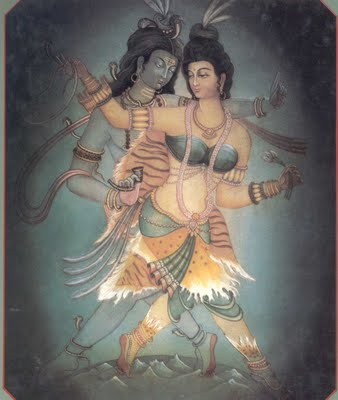
\includegraphics[scale=.3]{a20120304TheEternalWedding-img001.jpg}
\end{wrapfigure}
Is this at all clear? The Tantric path is easily confused with the pursuit of experiences that, despite their intensely pleasurable and ecstatic nature, are still no more than human, all too human. Ultimately, what is there to pursue since Atman, the unmoved mover, has no needs? There is nothing to seek, nothing to give up. All parts of existence provide us with the raw materials for transmutation, fuel for the awakening of the power of Shakti. The one thing necessary is to be ever vigilant, to be conscious of all that is moving, the images of Maya. That is to be as wise as the serpent.



\flrightit{Posted on 2012-03-04 by Cologero }

\begin{center}* * *\end{center}

\begin{footnotesize}\begin{sffamily}



\texttt{Matt on 2012-03-04 at 22:10 said: }

Yes, with all of Serrano's idiosyncrasies (the hidden nazi bases, ufo's, parallel universes etc.), he could be quite astute. He was also, to me at least, a great writer (even when his idiosyncrasies would reveal themselves and risk the coherency of his thought process). I found his writings to be very poetic. I read the Serpent of Paradise about 2 years ago at the bar/cafe at my university (ha I know, reading some Serrano at a university bar) after my classes were done for the week. I was so enthralled by it that I could not put it down and read it all the way through in that one sitting, never distracted by the chatter, hustle and bustle that went on all around me.

I think I'll revisit that book soon.


\end{sffamily}\end{footnotesize}

%de Giorgio
\section{The Alma Dancer}

Woman is not a “thing”, but an animal, which is worse: she is becoming a marionette, since that is what man liked. The aversion for woman, with that sacred fixation of “value”, is a modern obsession that proves the weakness of European man as ascetic and as warrior. The two attitudes that man should adopt before woman are all there: pure attitudes not dulled by rancor or bitterness.

\begin{wrapfigure}{rt}{.3\textwidth}
 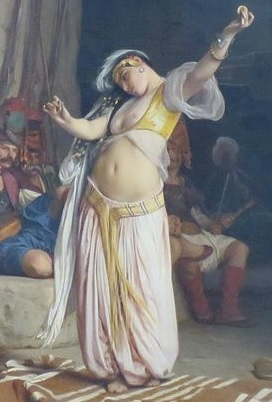
\includegraphics[scale=.5]{a20150517TheAlmaDancer-img001.jpg}
\caption{Alma Dancer}
\end{wrapfigure}

The Easterner, unlike a vulgar man, sees things differently: he knows that woman is a being whose superiority is obvious in a domain where man is very poor: freedom — although without light and without consciousness like children — an absence of prejudices, miraculous clarity, and a smile that man calls “evil”; not affirmation, but a shrug of the shoulder in the face of what man builds in a bourgeois way; to be capable of everything, accessible to everything, the receptacle of everything, bottomless, symbol of the cosmic matrix, insatiable. The Easterner, who is man in an absolute sense that the Westerner does not know, owes that to the fact that he is also woman, a thing that the Westerner will never know how to be.

That is why the Easterner is exquisite with woman; he caresses her, kills her, and confines her. He gives her, in short, her true freedom, her real strength. Taken such as she is, and not as man constructs her, woman has a value and that is why divinity gave her that miraculous thing which is the dance: the rhythm of her hip, the song the crowns the rhythm, the smile of evasion that is found only in the Ascetic who swims and empties himself: that smile that in maithuna [sexual union in Tantra] man does not have and only woman has, and who, speaking aesthetically, is visible only on certain Khemer heads. And I never saw the outcrop of the inexpressible change so well in plastic fixation except on those Khmer stones, and in the sculpture of Ellora, absolute figuration of absolute conjunction and absolute integration — beatitude, ananda.

That is the smile that woman, the sleeping child, and the Ascetic have: man attains this smile only when the infusion is absolute, when the sea overflows the rivers and waters. The Easterners see things thus, they can only see things thus.

At the time of medieval Chivalry, there was in man — this is mathematically certain — a freedom that he no longer has, and in woman, a submission and a sweetness that she can find again today only if man becomes again simple man, that is to say, more woman. Let Man be woman, and we will see what woman will become: a very fertile, docile, subtle being. At present the European is a Male and woman a Female wearing the mask of the Male. But man truly man (the East) more feminine than woman, subtle, ophidian, makes woman become again what she is.

Practically: let woman no longer roam about, let her be locked up, let her be respected; let what Westerners call “corruption” be, not exterior and visible, but confined — therefore free, not traditional. Women in the house and men outside: and you will see the action of woman — Dionysian, dissolving, Maenad-like action — recover her ancient strength.

In regard to the woman, the Islamic system was complete, whole. In Europe, the situation is horrendous: man pushes woman into the street, removes her veil, prostitutes her in sunlight, places her where she cannot be, where it is against nature for her to be: in the schools, trains, cafes, in the pigsty. The Anglo-Saxon peoples wanted that: and among us, with the stupidity that pushes us toward the ordure, we are following the example of those coarse beasts.

One final observation: the dance is solo (Oriental dance: the belly dance): Europe destroyed that, too, and introduced the couple's dance. If we follow the thread of this thought, we will go very far in the vision of Western perversion.


\hfill

\textbf{Guido De Giorgio}'s essay \textit{Short Notes on Ascesis and Anti-Europe}\footnote{\url{https://www.gornahoor.net/?p=6397}} is missing a note. Although this section was present in the original Ur journal and even the first collections, it was excluded in all the editions after 1955. I don't know why.

This note is collected in \textit{L'Instant et l'Eternité}. It appeared just before the incident about the sirocco in Tunisia. It extols the Traditional role of woman, particularly as it was, and might still be, found in Islamic nations.



\flrightit{Posted on 2013-05-17 by Cologero }

\begin{center}* * *\end{center}

\begin{footnotesize}\begin{sffamily}



\texttt{Saladin on 2013-05-21 at 22:46 said: }

while agreeing with De Giorgio's tenants and his overall Weltanschauung, I understand why these paragraphs were omitted. They are totally confusing (at least to me).


\hfill

\texttt{Cologero on 2013-05-21 at 23:25 said: }

Saladin, is the incomprehension the fault of the translation? If any passages are unclear, I can take another try at them.


\hfill

\texttt{Saladin on 2013-05-23 at 19:51 said: }

I doubt it is due to translation (and let me thank you once more for all the precious translations you have made available). In my humble opinion the passages do not completely make sense.

Take for example this paragraph: “The Easterner sees things differently: he knows that woman is, opposite vulgar man, a being whose superiority is obvious in a domain where man is very poor: freedom—although without light and without consciousness like children—an absence of prejudices, miraculous clarity, and a smile that man calls “evil”.

What does De Giorgio really wants to convey? That woman is more liberated (in spiritual sense) and less prejudiced? Cologero, I am sure you have a better grasp of what De Giorgio wants to convey here. Maybe you can clarify and comment on these passages which will be very much appreciated.

I really enjoyed your other translations of De Giorgio and I can only think that he himself decided that above note was not entirely coherent and he decided to omit from subsequent editions.

What does he really mean when he say: “Let Man be woman, and we will see what woman will become: a very fertile, docile, subtle being.”?


\hfill

\texttt{Mihai on 2013-05-24 at 03:42 said: }

I have read somewhere a comment by Evola in which he describes DeGiorgio as a “chaotic type of initiate”. I really wondered what he meant by that, but now, like you, I know.

\hfill

\texttt{Saladin on 2013-05-24 at 19:15 said: }

I had read that same comment (I am pretty sure on this blog) by Evola but totally forgotten it. However, granted De Giorgio may not be as lucid as Evola but I think he is nevertheless Traditional and immensely interesting.


\end{sffamily}\end{footnotesize}


\chapter{Arts and Poetry about Love}

\chapter{Sparse notes}
\section{Tales from the Anima}

\begin{quotex}

\textbf{Sehnsucht} is the inconsolable longing in the heart for we know not what. … [It is] that unnameable something, desire for which pierces us like a rapier at the smell of bonfire, the sound of wild ducks flying overhead, the title of \emph{The Well at the World's End}, the opening lines of \emph{Kubla Khan}, the morning cobwebs in late summer, or the noise of falling waves. \flright{\textsc{C S Lewis}}

You know that you love someone when you have glimpsed in her something too beautiful to die. \flright{\textsc{Gabriel Marcel}}

Ye who believe in affection that hopes, and endures, and is patient,

Ye who believe in the beauty and strength of woman's devotion,

List to the mournful tradition still sung by the pines of the forest;

List to a Tale of Love in Acadie, home of the happy. \flright{\textsc{Henry Wadsworth Longfellow}, \emph{Evangeline}}

\end{quotex}
Last night, I had another in a long series of dreams about the Anima. Our lovemaking was so sweet and enduring that we even spent time together afterwards; that is atypical. I even saw her face, which I had never clearly seen before. She was cute and somewhat petite. After three days together, I asked her if it was too soon to discuss marriage. Never before had marriage ever come up in a dream conversation. It was so disappointing to awaken. I never heard her answer.

\paragraph{Arabian Nights}
An unknown friend just sent me by post the tales of the 1001 Nights, but he neglected to send me a woman as creative as Scheherazade to read them to me. The stories have an urgency, when you consider that they represent a matter of life and death. Now I wonder what it would be like to spend 1001 nights with such a woman.

\begin{wrapfigure}{rt}{.3\textwidth}
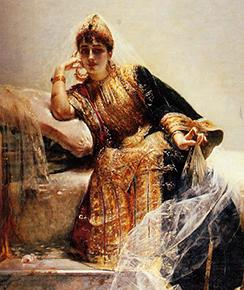
\includegraphics[scale=.5]{a20201115TalesfromtheAnima-img001.jpg} 
\caption{Scheherazade}
\end{wrapfigure}

Fearful that she would be unfaithful to him, the King married a new virgin every day, only to have her beheaded the next morning. Eventually, the kingdom ran out of virgins. The vizier's daughter, Scheherazade, volunteered to be the king's bride, to her father's consternation. But Scheherazade was quite intelligent and cultured. She had read widely in history, poetry, philosophy, science, and the arts. So on their first night together, she told the king a story, but did not finish it. Curious to hear the ending, he kept her a second night. Scheherazade finished the first story and started a second, again without finishing it. This continued for 1001 nights, at which point he admitted that he had fallen in love with her and spared her life.

Esoterically, Scheherazade risks her personal life to gain her immortal life with the king.

\paragraph{Worthiness of Love}
Frithjof Schuon points out that, according to an Hadith, \textbf{women, perfumes, and prayer} are worthy of love. Schuon explains why:

\begin{itemize}
\item \textbf{Woman}, synthesizing in her substance virgin nature, the sanctuary and spiritual company, is for man what is most lovable; in her highest aspect, she is the formal projection of merciful and infinite Inwardness in the outward; and in this regard she assumes a quasi-sacramental and liberating function. 
\item \textbf{Perfumes} represent qualities or beauties that are formless, exactly in the same way as music; that is to say that side by side with the formal projection of Inwardness, there exists also a complementary formless projection, symbolized, not by visual or tangible qualities, but by auditory and olfactory ones; perfumes are silent music. 
\item \textbf{Prayer} leads from Outward to Inward, and both consecrates and transmutes the qualitative elements of the outward realm. 
\end{itemize}

\paragraph{My Imaginary Friend}
\begin{quotex}
There is only one her for each him. She has been singled out for him in each register of the universe. This cannot be changed because She is the Her who came out of Him. In the turning of the wheel of the Eternal Return, it is not always given for them to meet. One or other may arrive late or too early.

It should be known that, in reality, the solution is to be able to bring Her back to life, to resurrect her within his soul. \flright{\textit{Nos}}

\end{quotex}
Often impatient with the all too slow process, through dreams, of the revelation of Her, I take it upon myself to imagine Her through my own efforts. But the imagination cannot create ex nihilo, so it needs an inspiration to kick it off. There are some women who are so beautiful, that men may be affected physically just by gazing upon her. This is how \textbf{Dante} described Beatrice in \emph{La Vita Nuova}:

\begin{quotex}
she showed herself so gentle and so full of all perfection, that she bred in those who looked upon her a soothing quiet beyond any speech; neither could any look upon her without sighing immediately. 

\end{quotex}
Yet even the Girl from Ipanema made the men sigh whenever she passed by. So my imagination requires more, much more. Beatrice, for Dante, represented, not just Beauty, but, more importantly, Wisdom. She guides him through the heavenly spheres toward God, something which the philosophers could not do.

Beyond a physical sigh, there is a spiritual sigh. Like Scheherazade, the image would be someone of high intellect, familiar with “history, poetry, philosophy, science, and the arts”; she would understand the transcendent meaning behind the appearances, often described in terms of the archetypes of the gods and goddesses.

And she is passionate about her life. She is elegant with refined tastes in fashion, art, architecture, perfumes. She intuitively grasps the rhythms of life, knowing when to dance and when to be still, just contemplating the world around her.

She seems to be how I might imagine myself to be, were I a woman.

\paragraph{The Soul of a Woman}
Although a woman longs to be “known”, for a man to “get her”, she nevertheless keeps many things hidden. She will drop a clue from time to time, and these must be carefully attended to. Yet the more you penetrate, and the more you think you know, something is still off kilter. It is not like looking through a window, but rather “through” a mirror. Left becomes right, and right becomes left, which is disorientating long before you become fully aware of it.

Yet it is necessary, because a man's soul is deficient. A human being consists of the physical along with the three soul functions of Willing, Feeling, and Thinking. A man focuses on his physical prowess and intellectual skills, the two least permanent parts of the human being. The physical is left behind at death along with most of one's thoughts. Thoughts have no permanent value. Even such a master of thinking like Thomas Aquinas came to the realization that they are just “so much straw”. What you Will and what you deeply Feel (not feelings in the trivial sense used by the modern world), will follow you, so these faculties also need development.

A child comes into the world with just the Willing and Feeling functions. He has desires and there is no space between his Feelings and their outward expression. Only much later does he learn to think.

Women don't give up the Willing and Feeling functions so easily, so she can help him reclaim them.

There is a reason men fail at that task — fear. I can still remember the first time I tried to pick up a woman at a nightclub. I was so nervous, it took all my inner force to overcome the self-induced fear. Over time, it became easier and stress-free. Not necessarily good, since motives are not pure; nevertheless, more possibilities opened up to me, often in unexpected ways.

\paragraph{Case study: Lucy}
\begin{quotex}
I know that I will meet you again and that everything will happen once again exactly as it did a long time ago. Except that this time I will not allow you to die. I will hold you in my arms, defending you against the dark waters of death. 

\end{quotex}
Temptation can be spiritual or material. Lucy's was spiritual. I received a strange email, filled with incoherent rantings. I put it away, but got another a month later. This one I answered. Lucy was at a low point in life, desperate for help or reassurance. Clearly, her circle of intimates could not see it or could not help. I responded to the second one, as best I could. The White Knight could not deny a damsel in distress. That calmed her and she became more coherent; we arranged for voice communication.

She turned out to be a woman of remarkable intelligence, deep spirituality, and a Sibylline visionary. She claimed to know my past and foresee my future. She suggested I was chosen to continue her spiritual tradition, which she offered to teach me. The spiritual turned into the personal, even becoming flirtatious. 

During our conversations, her most tender moments would melt my heart, but then she would go into an insane rage or enter into extended periods of inconsolable melancholy. Ultimately, she could not understand the possibility of a higher calling, so, like a dog returning to her vomit, she returned to the life circumstances that had caused her distress in the first place.

I was a failure, unable to defend her against the dark waters of death.

\paragraph{Case study: Harriett}
Harriett represents material temptation. She was raised in a Christian cult and her mother arranged her marriage. He left her with three children, leaving her burdened and alone. Yet she wanted to be known, and known intimately and completely; discussions about literature, films, metaphysics, religion, while suitable for me, just left her longing for more.

Harriett began mailing me her most intimate fantasies, amounting to several pages; they showed her to be highly intelligent and quite literate. There was a great attention to minute detail, including the scents of candles, titles of background music, clothing, the exact physical circumstances, the colour of the sky, lakes, streets, people, and so on.

Many were quite explicit, poetically describing the intensity of her felt desire and the physical sensations associated with lovemaking. Foreplay was also described in detail. She made no distinction between her experience of the physical and her inner feelings: “I wanted … to feel him touch the very core of my being.” No woman had ever spoken to me in such terms prior to that.

Other fantasies were so innocent and sweet, like her desire to make breakfast and have coffee on the patio with her lover. When we finally met, I was able to give her the XXX nights, but not the casual coffee in the morning. There was not enough physical attraction and I had no desire to raise another man's children. I expect to be fully punished for this in Purgatory.

\paragraph{Case study: Hafiz}
\begin{quotex}
Praise be to God what wonderful wealth is given to me tonight;

Because my Divine Beloved came to me, quite suddenly, tonight. 

\end{quotex}
Although born in modest circumstances, and working in a bakery by day, Hafiz studied assiduously at night. He taught himself law, science, maths, poetry. One day, he made a delivery to a wealthy household, where lived a young woman. Her beauty made him almost lose consciousness; he fell so madly in love, he could no longer eat and sleep normally. He wrote poems about her, despite his realization that she had been promised to another.

He vowed to keep a vigil of 40 nights at a saint's tomb, after which he would be granted his heart's desire. During one of his deliveries, she came out to meet him, having learned of his poems to her. She said she preferred a man of genius rather than the son of a king. Yet, he was so tired from his vigil, that he walked away.

On the 40th night, the archangel Gabriel came to fulfil the promises of the vigil. Suddenly, Hafiz realized that his heart's desire was for God, not for the woman.

This is what the 13th century Persian Sufi poet Hafiz has to say about self-emptying:

\textit{First, the self-emptying}:

\begin{quotex}
I Have Learned
So much from God
That I can no longer call myself
A Christian, a Hindu,
A Muslim, a Buddhist, a Jew.

The Truth has shared so much of Itself with me,
That I can no longer call myself
A man, a woman, an angel,
Or even pure Soul.

Love has befriended Hafiz so completely,
It has turned to ash,
And freed me
Of every concept and image
My mind has ever known.
\end{quotex}

\textit{To be followed by the feast!}

\begin{quotex}
Why
Just show you God’s menu?
Hell, we are all starving –
Let’s Eat!
\end{quotex}

The story of Hafiz’ awakening is a lesson in itself. It demonstrates the alchemical transformation of a soul from common desire to the gold of enlightenment:

When he was 21 and working as a baker’s assistant, Hafiz delivered some bread to a mansion and happened to catch a fleeting glimpse of a beautiful girl on the terrace. That one glimpse captured his heart, and he fell madly in love with her, though she did not even notice him. She was from a wealthy noble family and he was a poor baker’s assistant. She was beautiful, he was short and physically unattractive — the situation was hopeless.

As months went by, Hafiz made up poems and love songs celebrating her beauty and his longing for her. People heard him singing his poems and began to repeat them; the poems were so touching that they became popular all over Shiraz.

Hafiz was oblivious of his new fame as a poet; he thought only of his beloved. Desperate to win her, he undertook and arduous spiritual discipline that required him to keep a vigil at the tomb of a certain saint all night long for forty nights. It was said that anyone who could accomplish this near-impossible austerity would be granted his heart’s desire. Every day Hafiz went to work at the bakery. Every night he went to the saint’s tomb and stayed awake for this girl. His love was so strong that he succeeded in completing this vigil.

At daybreak on the fortieth day, the archangel Gabriel appeared before Hafiz and told him to ask for whatever he wished. Hafiz had never seen such a glorious, radiant being as Gabriel. He found himself thinking, “If God’s messenger is so beautiful, how much more beautiful must God be!” Gazing on the unimaginable splendor of God’s angel, Hafiz forgot all about the girl, his wish, everything. He said: “I want God!”

On this Easter weekend, I am also reflecting on the process of kenosis our self-emptying of all concepts, ideas, desires, mental superimpositions — to be followed by the fulfillment of a resurrection into a fuller, richer life.

\hfill

The incidents described are for illustrative purposes only, and should not be construed as descriptions of any incident or person, living or dead (apart, of course, for Hafiz).

\textit{Update 15 November 2022}: Probably the symbolism is buried too deep. Lucy and Harry are nicknames for Lucifer and Ahriman.


\flrightit{Posted on 2020-11-15 by Cologero }


\end{document}
